\def\GRAPHPATH{localgraphics}

\ifdefined\HANDOUT
  \documentclass[handout,aspectratio=1610,dvipsnames]{beamer}
  \def\GRAPHPATH{graphics}
\else
  \documentclass[aspectratio=1610,dvipsnames]{beamer}
\fi

\usepackage[margin=2cm]{geometry}
\usepackage[ngerman]{babel}

\usepackage{setspace}
\usepackage{booktabs}
\usepackage{array,graphics}
\usepackage{color}
\usepackage{soul}
\usepackage[linguistics]{forest}
\usepackage{multirow}
\usepackage{longtable}
\usepackage{langsci-gb4e}
\usepackage{soul}
\usepackage{enumitem}
\usepackage{ulem}
\usepackage{hyperref}
\usepackage{tikz}
\usetikzlibrary{arrows,positioning} 
\usepackage{lineno}
\usepackage{fontspec}
\usepackage{unicode-math}

\input{localcommands.tex}

\ifdefined\TITLE
  \title[Syntax | \StrSubstitute{\TITLE}{+}{ }]{Deutsche Syntax\\\StrSubstitute{\TITLE}{+}{ }}
\else
  \title[Deutsche Syntax]{Deutsche Syntax}
\fi

\author{Roland Schäfer}
\institute[FSU Jena]{Institut für Germanistische Sprachwissenschaft\\Friedrich-Schiller-Universität Jena}
\date[EGBD3]{\grau{stets aktuelle Fassungen: \url{https://github.com/rsling/VL-Deutsche-Syntax}}}

\begin{document}

\begingroup
  \setbeamertemplate{navigation symbols}{}
  \begin{frame}[noframenumbering,plain]
   \titlepage
  \end{frame}

  \begin{frame}{Inhalt}
    \centering 
    \scalebox{0.9}{\begin{minipage}{\textwidth}
      \begin{multicols}{2}
        \tableofcontents
      \end{multicols}
    \end{minipage}}
    \end{frame}
\endgroup

\ifdefined\TITLE
  \input{includes/\TITLE}
\else
  \section{Statistik, Inferenz und probabilistische Grammatik}
  \let\woopsi\section\let\section\subsection\let\subsection\subsubsection
  \section[Quantitativ]{Quantitative Analyse}

\begin{frame}
  {Übersicht}
  \begin{itemize}[<+->]
    \item Messungen und Experimente
    \item Hypothesen und Theorien
    \item Begriff der "`Variablen"'
    \item statistische Inferenz:
      \begin{itemize}[<+->]
	\item Hypothesenpaare H1 und H0
	\item Typ I- und Typ II-Fehler
	\item Validität
	\item exakte Hypothesentestung
      \end{itemize}
  \end{itemize}
\end{frame}

\begin{frame}
  {Literatur}
  \begin{itemize}
    \item \alert{\citet[Kap.\ 1 und 2]{MaxwellDelaney2004}}
    \item \citet[Kap.\ 1]{GravetterWallnau2007}
  \end{itemize}
\end{frame}

\subsection{Quantitative empirische Forschung}

\begin{frame}
  {Empirisch}
  \begin{itemize}[<+->]
    \item beobachtbare Phänomene
    \item Beobachtungen reproduzierbar
    \item messbar = beobachtbar (Sinneswahrnehmung an sich irrelevant)
    \item Realismus: "`wirkliche"' Phänomene und ihre Mechanismen
      \Zeile
    \item \alert{Experiment}
  \end{itemize}
\end{frame}

\begin{frame}
  {Empirie: Gründe für Reproduzierbarkeitsbedingung}
  \begin{itemize}[<+->]
    \item nicht-arbiträre Genauigkeit der Messung (Wirkung und Störeinflüsse)
    \item potentiell inadäquate Messung des theoretischen Konstrukts
    \item $\Rightarrow$ Vermeidung von Fehlschluss auf unechte Ursachen
    \item $\Rightarrow$ \alert{relevante Ursachen}
    \item Generalisierbarkeit der Ergebnisse
    \item Überkommen der individuell gefärbten Wahrnehmung
  \end{itemize}
\end{frame}

\begin{frame}
  {Individualgrammatik und fehlgeleitete Generative Grammatiker}
  \begin{itemize}[<+->]
    \item Gegenstand: interne (mentale) Grammatik (I-Grammatik)\\
      universeller und individueller Teil
    \item I-Grammatik bei jedem Sprecher (leicht) verschieden
    \item I-Grammatik erlaubt immer binäre Grammatikalitätsentscheidung
    \item also: \alert{Linguisten können eigene Grammatik untersuchen!}\\
      (Introspektion)
    \item universalistische Aussagen auf Basis solcher Ergebnisse zulässig
    \item \alert{Das ist auf allen Ebenen eine Frechheit!}
  \end{itemize}
\end{frame}

\begin{frame}
  {Hypothesen}
  \begin{itemize}[<+->]
    \item Ursprung der Hypothesen: Theorien
    \item interessante Hypothesen:
      \begin{itemize}[<+->]
	\item Formulierung relevanter Kausationsbedingung (wenn, dann)
	\item großer Gültigkeitsbereich (ein Sprecher vs.\ alle Sprecher)
      \end{itemize}
  \end{itemize}
\end{frame}

\begin{frame}
  {Hypothesenprüfung}
  \begin{itemize}[<+->]
    \item Kann die Hypothese weiter angenommen werden,\\
      oder liefert das Experiment starke Evidenz gegen sie?
    \item Probleme bei Prüfung:
      \begin{itemize}[<+->]
	\item störende Einflüsse
	\item ungenaue Operationalisierung (s.\,u.)
	\item stochastische Natur des Phänomens
	\item kleine Stichprobe (s.\,u.)
      \end{itemize}
    \item falsche Positive und falsche Negative jeweils zu vermeiden
  \end{itemize}
\end{frame}

\begin{frame}
  {Qualitative Forschung}
  \begin{itemize}[<+->]
    \item Daten besorgen\slash Experiment machen
    \item typischerweise \alert{kleine Datenmengen}
    \item Datenbetrachtung durch menschliche Wahrnehmung
    \item Interpretation der Daten durch Nachdenken
      \Zeile
    \item extrem fehleranfällig (Fehler = unzulässige Generalisierung)
    \item wichtig zur Hypothesengenerierung
  \end{itemize}
\end{frame}

\begin{frame}
  {Quantitative Forschung}
  \begin{itemize}[<+->]
    \item Daten besorgen\slash Experiment machen
    \item typischerweise \alert{größere Datenmengen}
    \item Datenanalyse durch Visualisierung\slash mathematische Datenbeschreibung
    \item Hypothesenprüfung durch \alert{Testverfahren} (s.\,u.)
    \item Grundlage moderner Wissenschaft
  \end{itemize}
\end{frame}

\begin{frame}
  {Operationalisierung, Theorie und Auxiliarhypothesen}
  \begin{itemize}[<+->]
    \item Operationalisierung = präzise Formulierung der Messmethode\\
      für ein theoretisches Konstrukt
    \item Bsp.\ Konstruk "`Satzlänge"': Wortanzahl? Phonemanzahl? Phrasenanzahl?
    \item Bsp.\ Konstrukt "`Satztopik"': Oha!?! \citep{CookBildhauer2013}
    \item alle genannten Beispiele: \alert{abhängig von Auxiliarhypothesen}\\
      bzw.\ anderen theoretischen Konstrukten (Wort, Phonem, Phrase, \dots)
  \end{itemize}
\end{frame}

\subsection{Grundbegriffe der quantitativen Forschung}

\begin{frame}
  {Grundgesamtheit}
  \begin{itemize}[<+->]
    \item von Interesse: allgemeine Gesetzmäßigkeiten
    \item also Untersuchungsgegenstand: \alert{alle X} (Sprecher, Sätze, \dots)
    \item untersuchbar: kleine Menge von X
    \item wenn "`alle X"' an sich sowieso sehr klein:\\
      interessante Fragestellung nur schwer möglich
      \Zeile
    \item fiktives Beispiel:
      \begin{itemize}[<+->]
	\item Sprecher ohne Ersatzinfinitiv (\textit{dass ich schlafen gemusst habe})\\
	  benutzen Modalverben öfter im Präteritum (\textit{dass ich schlafen musste})
	\item \dots aber es gibt nur einen Sprecher ohne Ersatzinfinitiv
	\item $\Rightarrow$ dann auch kein Theorie- und Empiriebedarf
      \end{itemize}
  \end{itemize}
\end{frame}

\begin{frame}
  {Stichprobe}
  \begin{itemize}[<+->]
    \item weil Grundgesamtheit intrinsisch nicht betrachtbar:\\
      \alert{Verwendung eingeschränkter Datensätze}
    \item ideal: \alert{uniform zufällige Stichprobe}\\
      = jedes Element der Grundgesamtheit hat die gleiche Chance beim Ziehen\\
    \item andere Möglichkeit: \alert{stratifizierte Stichprobe}\\
      = Stichprobe so zusammengesetzt, dass wichtige Eigenschaften\\
      proportional repräsentiert sind
    \item Problem bei Letzterem: haufenweise Auxiliarhypothesen
    \item außerdem: nicht unbedingt erforderlich, s.\ letzten Teil der heutigen VL
  \end{itemize}
\end{frame}

\begin{frame}
  {Induktive Inferenz}
  \begin{itemize}[<+->]
    \item Ziel: Schluss von Stichprobe auf Grundgesamtheit
    \item kritisch: Stichprobengröße
    \item Kriterium: Wahrscheinlichkeit, das Ergebnis per Zufall zu bekommen
    \item starker Einfluss: Stärke des Effekts in der Stichprobe
  \end{itemize}
\end{frame}

\begin{frame}
  {Variablen I}
  \begin{itemize}[<+->]
    \item meist uninteressanter Typ Fragestellung:\\
      "`Wieviel Prozent X haben Eigenschaft A?"'
    \item wegen \alert{Fehlens kausaler Zusammenhänge}
    \item Bsp.: wie oft \textit{wegen} mit Dat bzw.\ Gen?
    \item besser:\\
      \alert{"`Hängt bei X die Wahrscheinlichkeit für Eigenschaft B von A ab?"'}
    \item Bsp.: "`Nehmen denominale Präp eher Gen oder Dat?"'
  \end{itemize}
  \pause
  \begin{center}
    konzeptuell:
    \scalebox{0.7}{
      \begin{tabular}[h!]{|c||c|c|}
	\cline{2-3}
	\multicolumn{1}{c||}{} & denominale P & andere P \\
	\hline
	\hline
	Dat & $x_1$ & $x_2$\\
	\hline
	Gen & $x_3$ & $x_4$\\
	\hline
      \end{tabular}
    }
  \end{center}
\end{frame}

\begin{frame}
  {Variablen II}
  \begin{itemize}[<+->]
    \item Eigenschaften, quantitativ gemessen: \alert{Variablen}
    \item im Experiment:
      \begin{itemize}[<+->]
	\item \alert{kontrolliere} für Theorie irrelevante Variablen (\alert{Störvariablen})
	\item \alert{variiere} "`Ursachen-Variablen"' (\alert{unabhängige Variablen})
	\item \alert{beobachte} "`Wirkung-Variablen"' (\alert{abhängige Variablen})
      \end{itemize}
  \end{itemize}
\end{frame}

\begin{frame}
  {Experiment und Quasi-Experiment}
  \begin{itemize}[<+->]
    \item Problem in Astronomie, Korpuslinguistik usw.: keine Experimente möglich
    \item \alert{unabhängige Variablen nicht variierbar}
    \item Daten liegen bereits vor bzw.\ fallen vom Himmel
    \item Auswahl von Datensätzen, so dass von den unabhängigen Variablen\\
      die zur Theorieprüfung nötigen Permutationen im Datensatz vorkommen
    \item dabei Zusatzproblem bei Korpuslinguistik: Korpus meist nicht\\
      das eigene, wenig Informationen über mögliche Verzerrungen
      \Zeile
    \item \alert{Was ist die Grundgesamtheit?}
  \end{itemize}
\end{frame}

\begin{frame}
  {Hypothesenpaare}
  \begin{itemize}[<+->]
    \item \alert{H1 (eigene Hypothese)}:\\
      erwarteter Variablenzusammenhang aus Kausalrelation
    \item \alert{H0 (Nullhypothese)}: Negation der H1
    \item Ziel der Inferenzstatistik: \alert{Zurückweisung der H0}
    \item Logik: \textit{Entweder ein sehr seltenes Ereignis ist eingetreten,\\
      oder es besteht tatsächlich ein Zusammenhang.}
    \item $\Rightarrow$ Stärkung der H1, aber \alert{nicht "`Beweis"'}!
      \vspace{\baselineskip}
    \item geringe Bedeutung für sich genommen
    \item \alert{Severity} hängt von viel mehr Faktoren ab (Mayo)
    \item weitere Experimente\slash Replikationen
  \end{itemize}
\end{frame}

\begin{frame}
  {Mayos Strong Severity Principle}
      \vspace{\baselineskip}
  \begin{quote}
    \textit{Severity (strong): We have evidence for a claim C just to the extent it survives a stringent scrutiny.} If C passes a test that was highly capable of finding flaws or discrepancies from C, and yet none or few are found, then the passing result, \textbf{x}, is evidence for C. [Mayo 2018:14]
  \end{quote}
\end{frame}

\begin{frame}
  {Gerichtete Hypothesen}
  \begin{itemize}[<+->]
    \item übliche Hypothesen (H1):\\
      "`Es besteht ein Zusammenhang zwischen A und B."'
    \item H0 dann: Fehlen des Zusammenhangs
    \item = \alert{ungerichtete Hypothese}
    \item gerichtete Version: Benennung des genauen numerischen Zusammenhangs
    \item gerichtete Hypothesen: stärkere Aussage, schwerer zu zeigen,\\
      immer noch kein "`Beweis"'
  \end{itemize}
\end{frame}

\begin{frame}
  {Typ I- und Typ II-Fehler}
  \begin{itemize}[<+->]
    \item je nach
      \begin{itemize}[<+->]
	\item \alert{Stärke des Effekts}
	\item \alert{Homogenität} der Grundgesamtheit\slash Stichprobe
	\item \alert{Stichprobengröße}
      \end{itemize}
    \item Gefahr zweier möglicher Inferenzfehler:
      \begin{itemize}[<+->]
	\item \alert{Typ I ($\alpha$)}: H0 wird fälschlicherweise zurückgewiesen
	\item \alert{Typ II ($\beta$)}: H0 fälschlicherweise \alert{nicht} zurückgewiesen
      \end{itemize}
    \item Typ II-Fehler mehr gefürchtet, weil Artikel dann nicht angenommen wird
    \item inhaltlich beide gleich schwerwiegend
  \end{itemize}
\end{frame}

\begin{frame}
  {$\alpha$-Niveau und Teststärke}
  \begin{itemize}
    \item Logik der Hypothesenprüfung (genauer):\\
      Das Testergebnis ist so unwahrscheinlich per Zufall (H0) zu erzielen,\\
      dass H1 plausibel ist.
    \item die akzeptierte Schranke: \alert{$\alpha$-Niveau}
    \item Linguistik\slash Sozialwissenschaften: \alert{$\alpha=0.05$}
    \item wenn erreicht, gilt: \alert{Wenn in der GG der Zusammenhang nicht besteht,\\
      würde man nur in einer von 20 Stichproben die beobachtete Verteilung erwarten.}
      \Zeile
    \item \textit{If I tell you, you have a 5\% chance of being shot when you walk through the door, you go through the window.}
      \Zeile
    \item $\alpha$=Häufigkeit, mit der man sich langfristig positiv irrt\\
      (H0 korrekt, aber zurückgewiesen)
    \item vs.\ \alert{Teststärke}: $\beta$=Häufigkeit, mit der man sich langfristig negativ irrt\\
      (H0 falsch, aber nicht zurückgewiesen)
  \end{itemize}
\end{frame}

\subsection{Validität}

\begin{frame}
  {Statistische Validität}
  Gefahren für Typ I\slash II-Fehler
  \begin{itemize}[<+->]
    \item math.\ Bedingungen für Test nicht erfüllt (Typ I)
    \item kumulierter $\alpha$-Fehler (Typ I, s.\ nächste Folie)
    \item kleine Stichprobe (Typ II)
    \item zu große Variantion in der GG (Typ II)
      \Zeile
    \item in Korpora: schlechte Zusammensetzung des Korpus\\
      $\Rightarrow$ Phänomen mit mangelhafter Dispersion (Typ I)
  \end{itemize}
\end{frame}

%\begin{frame}
%  {$\alpha$-Kumulation}
%  \begin{itemize}[<+->]
%    \item Haupt-Hypothese H zerlegt in mehrere Teilhypothesen H1a, H1b, H1c
%    \item getestet mit gleichem Test an gleichem Datensatz
%    \item bei $\alpha$=0.05:
%      \begin{itemize}[<+->]
%	\item P(bestätige H1a|H0)=0.05
%	\item P(bestätige H1b|H0)=0.05
%	\item P(bestätige H1c|H0)=0.05
%	\item \alert{P(bestätige H1|H0)=\\
%	  P(bestätige H1a|H0)+P(bestätige H1b|H0)+P(bestätige H1c|H0)=0.15}
%      \end{itemize}
%    \item anders gesagt: Jede einzelne H1 wird bei $\alpha=0.05$ in einem von 20 Fällen fälschlicherweise bestätigt, aber für die gesamte H1 haben wir drei Testfälle produziert.
%    \item $\alpha$-Fehlerwahrscheinlichkeit steigt also auf $0.15$\\
%      \alert{einer von 6.67 Tests mit Typ I-Fehler}
%  \end{itemize}
%\end{frame}

\begin{frame}
  {Interne Validität}
  \begin{itemize}[<+->]
    \item Irrtum beim Herstellen des Kausalzusammenhangs
    \item Grund (Korpuslinguistik): verzerrte Stichprobenzusammensetzung
    \item Bsp.:
      \begin{itemize}[<+->]
	\item H1: Im DECOW2012 kommt öfter das Pronomen \textit{son} vor als im DWDS Kernkorpus, weil es erst nach 2000 zum eigenständigen Pronomen wurde.
	\item H0 wird auf Basis zweier Stichproben (DECOW2012, DWDS) zurückgewiesen.
	\item wirkliche Ursache: Registerunterschiede
      \end{itemize}
  \end{itemize}
\end{frame}

\begin{frame}
  {Validität des Konstrukts}
  \begin{itemize}[<+->]
    \item Korrektheit des theoretischen Konstrukts
    \item eigentlich aus der Psychologie
    \item aber riesiges mißachtetes Problem in der Linguistik
    \item Bsp.:
      \begin{itemize}
	\item Beobachtung: Das Deutsche bewahrt\\
	  genus-typische Pluralflexion am Substantiv.
	\item Konstrukt: Nominalklammer\slash Klammerprinzip\\
	  (NP-Kongruenzklammer Artikel--Substantiv, \citealt{Ronneberger2010})
	\item Hypothese zu Beobachtung: Flexionserhalt stärkt Klammerprinzip
	\item \alert{Das Konstrukt ist hochgradig beliebig und unterdefiniert.}
	\item \alert{Abhilfe: nur Konstrukte\slash Hypothesen,\\
	  die starke Vorhersagen generieren (s.\ Junggrammatiker)}
      \end{itemize}
  \end{itemize}
\end{frame}

\begin{frame}
  {Externe Validität}
  \begin{itemize}[<+->]
    \item Generalisierbarkeit der Ergebnisse (über Raum, Zeit usw.)
    \item Problem: zu große Homogenität der Stichprobe\\
      (was für statistische Validität wiederum gut ist)
    \item Bezug auf Korpora:
      \begin{itemize}[<+->]
	\item zu spezifische Stratifikation (DeReKo)
	\item verzerrte Stichprobe (evtl.\ traditionelle Webkorpora)
      \end{itemize}
  \end{itemize}
\end{frame}

\subsection{Ableitung des Fisher-Exakt-Tests aus ersten Prinzipien}

\begin{frame}
  {Ronald A.\ Fisher (1890--1962)}
  \begin{itemize}[<+->]
    \item Statistik als Teil der rationalen wissenschaftlichen Argumentation,\\
      der Interpretation von Experimenten
    \item daher: möglichst kein Mathematik-Jargon
    \item eingeschränkte Induktion als theoriegeleitete Dateninterpretation
    \item Kontrolle aller unabhängigen Variablen
    \item \alert{alle anderen (Stör-)Variablen konzeptuell zufallsgebunden}
  \end{itemize}
\end{frame}

\begin{frame}
  {Das Tassen-Problem}
  \begin{itemize}[<+->]
    \item Behauptung: Dame X kann am Geschmack erkennen,\\
      ob der Tee oder die Milch zuerst in die Tasse gegossen wurde.
    \item prä-fishersches Konzept: \alert{alle Störvariablen kontrollieren}\\
      und gleich machen, sonst keine valide Inferenz möglich
    \item Fisher: Das ist prinzipiell unmöglich, umständlich, teuer, \alert{unnötig}!
    \item wenn alle irrelvanten Stör-Faktoren zufällig, dann:
      \begin{itemize}[<+->]
	\item Variiere die relevante unabhängige Variable.
	\item Vergleiche das Ergebnis mit zufällig erwartbaren Ergebnissen.
	\item \alert{Wie unwahrscheinlich ist das erzielte Ergebnis\\
	  unter der Zufallsannahme?}
      \end{itemize}
  \end{itemize}
\end{frame}

\begin{frame}
  {Wahrscheinlichkeiten, richtig zu raten}
  \begin{itemize}[<+->]
    \item acht Tassen (zwei Milch zuerst, zwei Tee zuerst)
    \item \alert{Mit wie vielen richtigen Treffern wären Sie zufrieden?}
      \pause
      \pause
    \item Es muss die Wahrscheinlichkeit errechnet werden,\\
      eine, zwei, drei oder vier Tassen richtig zu raten.
      \Zeile
    \item \alert{Typischerweise schätzen Menschen solche Kombinatorikprobleme\\
      intuitiv falsch ein.}
  \end{itemize}
\end{frame}

\begin{frame}
  {GENAU Richtig durch Zufall}
  \begin{equation}
    P(\mathsf{richtig\ per\ Zufall})=\frac{\mathsf{Anzahl\ richtiger\ Zuweisungen}}{\mathsf{Anzahl\ aller\ potentiellen\ Zuweisungen}}
  \end{equation}
  \pause
  \begin{itemize}[<+->]
    \item Anzahl richtiger Zuweisungen: 1
    \item mögliche Zuweisungen: einfaches kombinatorisches Problem
  \end{itemize}
\end{frame}

\begin{frame}
  {mögliche Zuweisung von acht Tassen zu Milch\slash Tee zuerst}
  \begin{itemize}[<+->]
    \item erste MZ-Tasse: eine von 8
    \item zweite MZ-Tasse: eine von 7
    \item dritte MZ-Tasse: eine von 6
    \item vierte MZ-Tasse: eine von 5
    \item fünfte MZ-Tasse: STOPP (automatisch TZ)
    \item \alert{Möglichkeiten, 4 Tassen aus 8 auszuwählen:\\
      $8\cdot7\cdot6\cdot5=1680$}
  \end{itemize}
\end{frame}

\begin{frame}
  {Reihenfolge egal}
  \begin{itemize}[<+->]
    \item bisher: jedes Set von 4 MZ-Tassen ist in verschiedenen Reihenfolgen\\
      in der Menge der Möglichkeiten
    \item \alert{Möglichkeiten, vier Tassen zu ordnen:\\
      $4\cdot3\cdot2\cdot1=24$}
      \Zeile
    \item Reihenfolge hier egal, also:
  \end{itemize}
  \pause
  \begin{equation}
    \mathsf{Anzahl\ aller\ potentiellen\ Zuweisungen}=\frac{1680}{24}=70
  \end{equation}
\end{frame}

\begin{frame}
  {Wenn Dame X also genau richtig liegt}
  \begin{itemize}[<+->]
    \item per Zufall genau richtig:\\
      in einem von 70 Fällen, $p=0.014$
      \Zeile
    \item $\alpha$-Niveau von 0.05 also erreicht
  \end{itemize}
\end{frame}

\begin{frame}
  {Binomialkoeefizienten}
  \begin{itemize}[<+->]
    \item eigentlich \alert{Binomialkoeffizient}
    \item "`Lotto-Kombinationen"': $k$ aus $n$\\
      ohne Zurücklegen und ohne Beachtung der Reihenfolge
  \end{itemize}
  \Zeile
  \pause
  \begin{equation}
    \binom{n}{k}=\frac{n!}{k!(n-k)!}
  \end{equation}
\end{frame}

\begin{frame}
  {Kombinatorik für 3 richtige MZ}
  \begin{itemize}[<+->]
    \item die drei richtigen: $\binom{4}{3}$
    \item die eine falsche aus vier TZ: $\binom{4}{1}$
    \item Anzahl der Möglichkeiten drei richtige aus vier MZ\\
      und dann eine falsche aus vier TZ zu ziehen: $\binom{4}{3}\cdot\binom{4}{1}=4\cdot4=16$
  \end{itemize}
  \Zeile
  \pause
  \begin{equation}
    P(drei\ richtig\ per\ Zufall)=\frac{16}{70}=0.229
  \end{equation}
\end{frame}

\begin{frame}
  {Problem zu kleiner Stichproben}
  \begin{itemize}[<+->]
    \item \alert{Bei $\alpha=0.05$ reichen also drei richtige nicht im Ansatz!}
    \item alle schlechteren Ergebnisse: folglich auch nicht ausreichend
    \item Und bei 30 von 40 richtigen (also insgesamt 80 Tassen)?
  \end{itemize}
\end{frame}


\ifdefined\TITLE
  \section{Nächste Woche | Überblick}

  \begin{frame}
    {Einzelthemen}
    \begin{enumerate}
      \item Statistik, Inferenz und probabilistische Grammatik
      \item \alert{Deskriptive Statistik}
      \item Nichtparametrische Verfahren
      \item z-Test und t-Test
      \item ANOVA
      \item Freiheitsgrade und Effektstärken
      \item Power
      \item Lineare Modelle
      \item Generalisierte Lineare Modelle
      \item Gemischte Modelle
    \end{enumerate}
  \end{frame}
\fi


  \let\subsection\section\let\section\woopsi

  \section{Deskriptive Statistik}
  \let\woopsi\section\let\section\subsection\let\subsection\subsubsection
  
\begin{frame}
  {Übersicht}
  \begin{itemize}[<+->]
    \item Deskriptive Statistik als \alert{Aggregation von Daten}
      \Halbzeile
    \item Verteilungen in Stichproben und Grundgesamtheiten:
      \begin{itemize}
	\item Zentralmaße
	\item Streuung (Varianz)
      \end{itemize}
    \item \orongsch{Theoretische vs.\ empirische Verteilungen}
      \Halbzeile
    \item \alert{Kovarianz} | Miteinander variierende Variablen
      \Halbzeile
    \item \alert{Konfidenzintervalle} | Genauigkeiten von Schätzungen?
  \end{itemize}
\end{frame}

\begin{frame}
  {Literatur}
  \begin{itemize}
    \item Google, Stackoverflow usw.
      \Zeile
    \item \citet{GravetterWallnau2007}\\
      Achtung! \orongsch{Vermittelt eine falsche Philosophie bei Anwendung der Tests!}
      \Halbzeile
    \item \citet{Bortz2010}
  \end{itemize}
\end{frame}

\section{Motivation}

\begin{frame}
  {Zweck der deskriptiven Statistik}
  \begin{itemize}[<+->]
    \item Mit unbewaffnetem Auge auf Daten zu blicken, ist meistens zwecklos.
      \Halbzeile
    \item In Zahlen sehen Menschen nur schlecht Tendenzen und Zusammanhänge.
      \Zeile
    \item Deskriptive Statistik
      \begin{itemize}[<+->]
        \item \alert{Zusammenfassen}
        \item \alert{Gruppieren}
        \item \alert{Visualisieren}
      \end{itemize}
  \end{itemize}
\end{frame}


\begin{frame}
  {Was will man wissen?}
  \begin{itemize}[<+->]
    \item Definition der Grundgesamtheit
      \Halbzeile
    \item \alert{Stichprobengröße ($n$)}
      \begin{itemize}[<+->]
        \item 200 Sätze aus dem Korpus
        \item 1.000 Reaktionen (von 50 Probanden) im Experiment
        \item Was sind die elementaren gemessenen Datenpunkte?
      \end{itemize}
      \Halbzeile
    \item Stichprobenmethode
      \begin{itemize}[<+->]
        \item \alert{Zufallsstichprobe} | Nachweis der uniformen Zufälligkeit
        \item \alert{Quotenstichprobe} | Stratifzierung und Begründung
      \end{itemize}
  \end{itemize}
\end{frame}


\section{Skalenniveau}

\begin{frame}
  {Messvariablen und Skalenniveaus}
  \begin{itemize}[<+->]
    \item \alert{dichotom\slash binär} | \gruen{Menge $\{A, B\}$} | zwei disjunkte Kategorien\\
      \grau{männlich, weiblich ; Präteritum, Perfekt}
      \Viertelzeile
    \item \alert{nominal\slash kategorial} | \gruen{Menge $\{A, B, ..\}$} | disjunkte Kategorien\\
      \grau{Parteizugehörigkeit ; NP, AP, VP}
      \Viertelzeile
    \item \alert{ordinal} | \gruen{Tupel $\langle A, B, ..\rangle$, \rot{nicht} $\mathbb{N}$ oder $\mathbb{Z}$} | disjunkte Kategorien mit Rang\\
      \grau{Schulnoten ; 5- oder 7-Punkt-Skalen für Akzeptabilität}\\
      \Viertelzeile
    \item \alert{Verhältnis} | \gruen{$+\mathbb{Q}_0$} | geordnete Werte mit Nullpunkt\\
      \grau{Temperatur in Kelvin ; Lesezeiten}
      \Viertelzeile
    \item \alert{Intervall} | \gruen{$\mathbb{Q}$} | Wie Verhältnis, aber ohne Nullpunkt\\
      \grau{Temperatur in Celsius}
      \Zeile
    \item \rot{Zähldaten} | \rot{Keine} beobachtbaren Variablen, sondern\\
      Aggregation von dichtotomen, nominalen oder ordinalen Variablen\\
  \end{itemize}
\end{frame}

\begin{frame}
  {Intervalle vs.\ Verhältnisse}
  \begin{itemize}[<+->]
    \item \alert{Verhältnisskala} | Größe von Menschen in cm
      \begin{itemize}[<+->]
	\item $200 cm = 2 \times 100 cm$ usw.
	\item Keine Messung unter $0 cm$ 
      \end{itemize}
      \Zeile
    \item \alert{Intervallskala} | Dasselbe als \alert{Abweichung vom Mittel}
      \begin{itemize}[<+->]
	\item $4 cm = 2 \times 2 cm$ usw.
        \item \orongsch{$184 cm \neq 2 \times 182 cm$}
	\item Negative Messungen möglich
      \end{itemize}
  \end{itemize}
\end{frame}

\begin{frame}
  {Relevanz der Skalenniveaus}
  \begin{itemize}[<+->]
    \item Bestimmung \alert{zulässiger mathematischer Operationen}
      \Halbzeile
    \item \alert{Deskriptive Statistiken} je nach Skalenniveau
      \Halbzeile
    \item Zulässigkeit von \alert{inferenzstatistischen Tests} je nach Skalenniveau
  \end{itemize}
\end{frame}


\section{Zentraltendenz}

\begin{frame}
  {Zentraltendenz I}
  \alert{Modus} | Der \alert{häufigste Wert} | \orongsch{Alle Skalenniveaus}\\
  \Zeile
  \begin{center}
    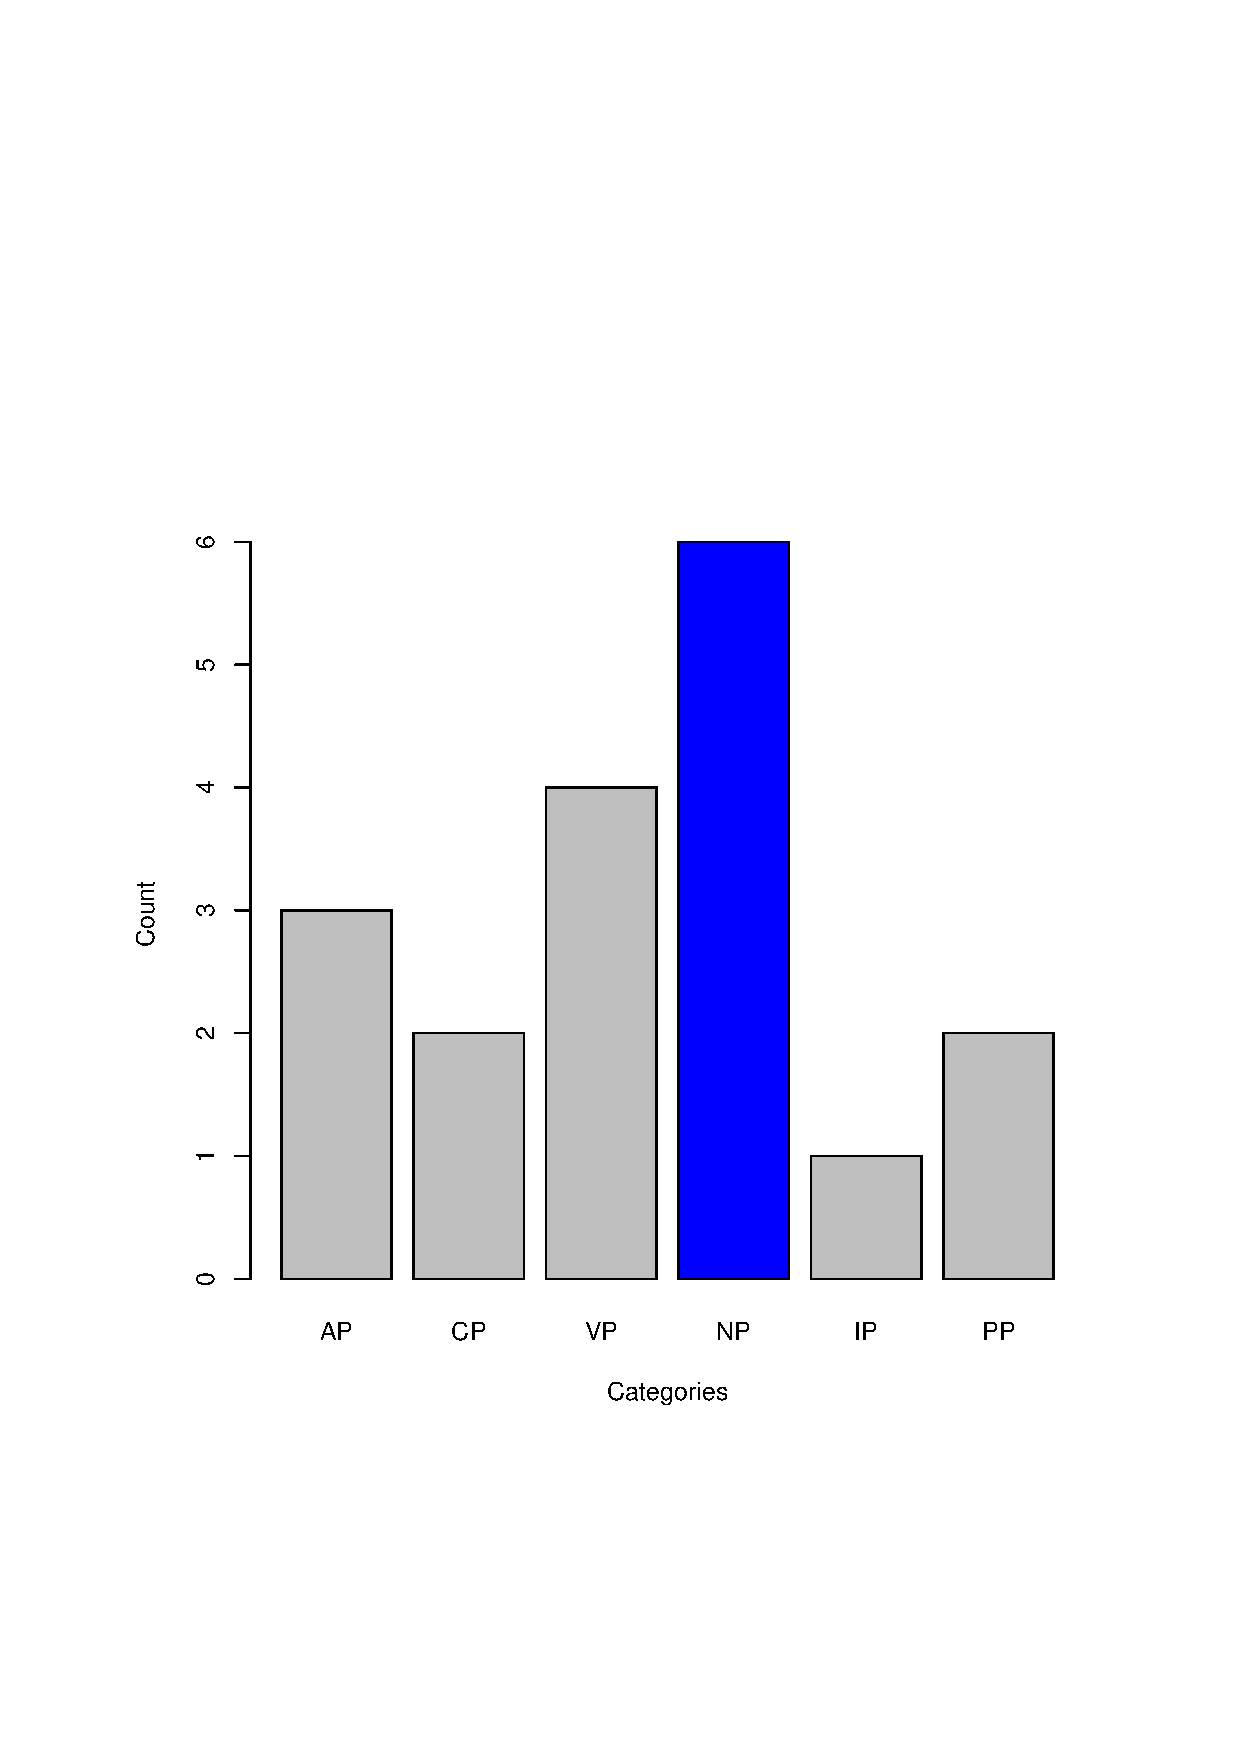
\includegraphics[height=0.6\textheight]{RVorlesung/mode}
  \end{center}
\end{frame}

\begin{frame}
  {Zentraltendenz II}
  \alert{Median} | \alert{Mitte der sortierten Stichprobe} | \orongsch{ab Ordinalskala}\\
  \Zeile
  \begin{center}
    \includegraphics[height=0.6\textheight]{RVorlesung/median}
  \end{center}
  \Zeile
  \grau{\footnotesize Numerische Messungen | Verschiedene Interpolationsmethoden\\
    \url{https://en.wikipedia.org/wiki/Quantile\#Estimating_quantiles_from_a_sample}}
\end{frame}

\begin{frame}
  {Median bestimmen | Stichprobe}
  \centering 
  \includegraphics[height=0.9\textheight]{RVorlesung/median1a}
\end{frame}

\begin{frame}
  {Median bestimmen | Sortierte Stichprobe}
  \centering 
  \includegraphics[height=0.9\textheight]{RVorlesung/median1b}
\end{frame}

\begin{frame}
  {Median bestimmen | Verzerrtere sortierte Stichprobe}
  \centering 
  \includegraphics[height=0.9\textheight]{RVorlesung/median2}
\end{frame}

\begin{frame}
  {Zentraltendenz III}
  \alert{Arithmetisches Mittel} $\bar{x}$ | Summe aller Werte geteilt durch $n$ | \orongsch{ab Intervallskala}\\
  \Zeile
  \begin{multicols}{2}
    \centering 
    \hspace{0em}\\
    \vspace{0.1\textheight}
    $\bar{x}=\frac{\sum\limits_{i=1}^{n}x_i}{n}$
    \newpage
    \raggedright
    \includegraphics[height=0.6\textheight]{RVorlesung/mean}
  \end{multicols}
\end{frame}



\section{Empirische Verteilungen und Dispersion}

\begin{frame}
  {Warum sind Dispersionsmaße wichtig?}
  \alert{Dispersion} | Streuung der Daten\\
  \Zeile
  \begin{itemize}[<+->]
    \item \alert{Zentraltendenz} | Orientierung über Tendenzen der Stichprobe
     \Zeile 
    \item \alert{Ein Maß für Zentraltendenz} für \orongsch{beliebig viele Verteilungsformen}
      \Halbzeile
    \item Arithmetisches Mittel | deskriptiv oft \orongsch{unbrauchbar ohne Betrachtung der Verteilung}
    \item Median | \orongsch{auch nur bedingt besser}
  \end{itemize}
\end{frame}

\begin{frame}
  {Vier sortierte Stichproben}
  Jeder Punkt entspricht einem Datenpunkt\slash einer Messung!\\
  \begin{center}
    \includegraphics[height=0.75\textheight]{RVorlesung/foursamples}
  \end{center}
\end{frame}

\begin{frame}
  {Verteilungsformen}
  \alert{Histogramme} | Vier Stichproben mit \alert{$\bar{x}=3.72$} und \alert{$n=18$}\\
  \Viertelzeile
  \grau{Zum Beispiel 18 Bewertungen eines Probanden auf einer 7-Punkt-Skala}\\
  \begin{center}
    \includegraphics[height=0.75\textheight]{RVorlesung/fourdists}
  \end{center}
\end{frame}

\begin{frame}
  {Quartile}
  \alert{Quartile} | Generalisierung des Medians (bei 25 \%, 50 \%, 75 \%)\\
  \begin{center}
    \includegraphics[height=0.85\textheight]{RVorlesung/fourquartiles}
  \end{center}
\end{frame}


\begin{frame}
  {Interquartilbereich, Boxplots und Violinplots}
  \begin{itemize}[<+->]
    \item Interquartilbereich \alert{$IQR = Q_3-Q_1$} | Die mittleren 50 \%
     \Zeile 
    \item Boxplots
      \Viertelzeile
      \begin{itemize}[<+->]
        \item \alert{Median} | Linie in der Mitte
        \item \alert{Oberes und unteres Quartil} | Boxen
        \item \alert{1,5-facher Interquartilabstand} | gestrichelte Hebel
        \item \alert{Ausreißer} | Punkte
      \end{itemize}
      \Halbzeile
    \item Violinplots | Zusätzlich Plot der Verteilungsdichte (statt Box)
  \end{itemize}
\end{frame}


\begin{frame}
  {Boxplots | Die bessere Zusammenfassung}
  \begin{center}
    \includegraphics[height=0.7\textheight]{RVorlesung/fourbox}
  \end{center}
\end{frame}


\begin{frame}
  {Violinplots | Die noch bessere Zusammenfassung}
  \begin{center}
    \includegraphics[height=0.7\textheight]{RVorlesung/fourviolins}
  \end{center}
\end{frame}

\begin{frame}
  {Was bestimmt die Varianz?}
  Die \alert{Distanzen der Messwerte zum Mittel} sind unterschiedlich groß.\\
  \begin{center}
    \includegraphics[height=0.7\textheight]{RVorlesung/fourvariances}
  \end{center}
\end{frame}


\begin{frame}
  {Varianz und Standardabweichung}
  \alert{Varianz $s^2$} | Quadrierte \alert{mittlere Abweichung} vom Mittelwert\\
      \begin{center}
	\alert{$s^2(x)=\frac{ \sum\limits_{i=1}^{n}(x_i-\bar{x})^2}{n-1}$}
      \end{center}
\pause
      \vspace{0.5cm}
    \alert{Standardabweichung $s$} | Quadratwurzel der Varianz\\
      \begin{center}
	\alert{$s(x)=\sqrt{s^2(x)}$}
      \end{center}
      \vspace{0.5cm}

  \pause
    \alert{Summe der Quadrate} | Zählerterm der Varianz\\
  \begin{center}
    $SQ(x)=\sum\limits_{i=1}^{n}(x_i-\bar{x})^2$
  \end{center}
\end{frame}

\begin{frame}
  {Unterschiedliche Standardabweichungen}
  \begin{center}
    \includegraphics[height=0.9\textheight]{RVorlesung/stdevs}
  \end{center}
\end{frame}


\begin{frame}
  {z-Wert}
  Für jeden Messpunkt $x_i$ | \alert{$z_i=\frac{x_i-\bar{x}}{s(x)}$}\\
  \begin{center}
    \includegraphics[height=0.8\textheight]{RVorlesung/fourzs}
  \end{center}
\end{frame}

\begin{frame}
  {z-Wert | Rechenbeispiel}
  \begin{itemize}[<+->]
    \item Bsp.: $\alert{x}=[3.9, 4.3, 7.2, 8.5, 11.1, 12.1, 14.0, 20.7]$
      \Halbzeile
      \begin{itemize}[<+->]
        \item $\alert{\bar{x}}=$\onslide<2->{$10.225$}
          \Halbzeile
        \item $\alert{s^2(x)}=$$\frac{(3.9-10.255)^2+\ldots+(20.7-10.225)^2}{8-1}=$$\frac{215.495}{7}=$$30.785$
          \Halbzeile
        \item $\alert{s(x)}=$$\sqrt{30.785}=$$5.548$
          \Halbzeile
        \item $\alert{z}=[\frac{3.9-10.225}{5.548}$, \ldots, $\frac{20.7-10.225}{5.548}]=$$[-1.140, -1.068, -0.545, -0.311, 0.158, 0.338, 0.680, 1.888]$
      \end{itemize}
  \end{itemize}
\end{frame}

\section{Bivariate Statistiken}

\begin{frame}
  {Zähldaten von zwei Variablen}
  \alert{Kreuztabelle} | Darstellung der Zähldaten zweier Variablen\\
  \Zeile
  \begin{center}
    \begin{tabular}{rcc}
      \cline{2-3}
      &&\\
      & \textbf{Variable 1 | Wert 1} & \textbf{Wert2} \\
      &&\\
      \hline
      &&\\
      \textbf{Variable 2 | Wert 1} & Anzahl $x_{11}$ & Anzahl $x_{12}$ \\
      &&\\
      \textbf{Wert 2} & Anzahl $x_{21}$ & Anzahl $x_{22}$ \\
      &&\\
      \hline
    \end{tabular}
  \end{center}
\end{frame}

\begin{frame}
  {Korrelationen | Zusammenhänge zwischen numerischen Variablen}
  Bivariate Korrelationskoeffizienten | \orongsch{ab Ordinalskala}\\
  \begin{center}
    \includegraphics[height=0.7\textheight]{graphics/corrplot}
  \end{center}
\end{frame}


\begin{frame}
  {Kovarianz | Illustration 1}
  Koordinate von $\langle\bar{x},\bar{y}\rangle$ | Mittel der beiden gemessenen Variablen\\
  \begin{center}
    \includegraphics[height=0.7\textheight]{graphics/cov02}
  \end{center}
\end{frame}


\begin{frame}
  {Kovarianz | Illustration 2}
  Punktvarianzen | $x_3-\bar{x}=-7.81$ und $y_3-\bar{y}=-5.80$ | \alert{$-7.81\cdot-5.80=45.30$}\\
  \begin{center}
    \includegraphics[height=0.7\textheight]{graphics/cov03}
  \end{center}
\end{frame}


\begin{frame}
  {Kovarianz | Illustration 3}
  Punktvarianzen | $x_{17}-\bar{x}=4.95$ und $y_{17}-\bar{y}=7.11$ | \alert{$4.95\cdot7.11=35.19$}\\
  \begin{center}
    \includegraphics[height=0.7\textheight]{graphics/cov04}
  \end{center}
\end{frame}


\begin{frame}
  {Kovarianz | Illustration 4}
  Puntvarianzen für alle $\langle x_i,y_i\rangle$ \ $cov(x,y)=34.52$\\
  \begin{center}
    \includegraphics[height=0.7\textheight]{graphics/cov05}
  \end{center}
\end{frame}


\begin{frame}
  {Kovarianz | Illustration 5}
  Ausreißer bei ansonsten positiver Kovarianz | \alert{Negatives Produkt} der Punktvarianzen\\
  \begin{center}
    \includegraphics[height=0.7\textheight]{graphics/cov06}
  \end{center}
\end{frame}


\begin{frame}
  {Kovarianz | Illustration 6}
  Punktvarianzen | $x_{21}-\bar{x}=6.77$ und $y_{21}-\bar{y}=-8.79$ | \alert{$6.77\cdot-8.79=-59.51$}\\
  \begin{center}
    \includegraphics[height=0.7\textheight]{graphics/cov07}
  \end{center}
\end{frame}

\begin{frame}
  {Negative Kovarianz}
  Tendenziell negative Abhängigkeit | Punktvarianzen überwiegend | $cov(x,y)=-33.77$\\
  \begin{center}
    \includegraphics[height=0.7\textheight]{graphics/cov08}
  \end{center}
\end{frame}

\begin{frame}
  {Kovarianz nahe Null}
  Ohne Abhängigkeit | Kovarianz nahe 0 |$cov(x,y)=-1.74$\\
  \begin{center}
    \includegraphics[height=0.7\textheight]{graphics/cov09}
  \end{center}
\end{frame}

\begin{frame}
  {Kovarianz}
  \alert{Kovarianz} | Kombination der Abweichung der Messpunkte vom jeweiligen Mittel\\
  \begin{center}
    \alert{$cov(x,y)=\frac{\sum\limits_{i=1}^{n}(x_i-\bar{x})\cdot(y_i-\bar{y})}{n-1}$}\\
    \Halbzeile
    \alert{Summe der Produkte} | Der Zählerterm | $SP(x,y)=\sum\limits_{i=1}^{n}(x_i-\bar{x})\cdot(y_i-\bar{y})$
  \end{center}
  \Halbzeile
  \begin{itemize}[<+->]
    \item \gruen{$x_i-\bar{x}>0$} und \gruen{$y_i-\bar{y}>0$} | Beitrag zur Kovarianz \gruen{positiv}
    \item \orongsch{$x_i-\bar{x}<0$} und \orongsch{$y_i-\bar{y}<0$} | Beitrag zur Kovarianz \gruen{positiv}
      \Halbzeile
    \item \gruen{$x_i-\bar{x}>0$} und \orongsch{$y_i-\bar{y}<0$} | Beitrag zur Kovarianz \orongsch{negativ}
    \item \orongsch{$x_i-\bar{x}<0$} und \gruen{$y_i-\bar{y}>0$} | Beitrag zur Kovarianz \orongsch{negativ}
  \end{itemize}
\end{frame}



\begin{frame}
  {Korrelationskoeffizient}
  \alert{Korrelationskoeffizient} | Im Gegensatz zur Kovarianz \alert{skalenunabhängig}\\
  \vspace{3\baselineskip}
  \begin{center}
    $r(x,y)=\frac{cov(x,y)}{s(x)\cdot s(y)}$\\
    \Zeile
    \grau{Pearson-Korrelation}
  \end{center}
\end{frame}



\section{Standardfehler und Konfidenzintervalle}

\begin{frame}
  {Anteilswerte und Stichproben}
  \begin{itemize}[<+->]
    \item Das Verb \textit{essen} | Manchmal mit, manchmal ohne Akkusativ (direktes Objekt)
    \item Angenommenes wahres Verhältnis | \alert{Mit Objekt 39 \%, ohne Objekt 61 \%}
      \Halbzeile
    \item Viele Stichproben mit n=100 | Ergebnis \rot{nicht} immer 39 zu 61
     \Doppelzeile 
    \item \alert{95\%-Konfidenzintervall} | \gruen{In welchem Bereich liegen 95\% aller Messwerte bei n=100?}
    \item Güte von Stichproben einer bestimmten Größe angesichts gegebener Proportionen
  \end{itemize}
\end{frame}


\begin{frame}
  {Sechzehn simulierte Stichprobenentnahmen (n=100)}
  \centering 
  \includegraphics[height=0.8\textheight]{RVorlesung/sixteenbernoullis}
\end{frame}

\begin{frame}
  {Wiederholte Stichprobenentnahmen (n=100)}
  \centering 
  \includegraphics[width=0.3\textwidth]{RVorlesung/manybernoullis1}
  \includegraphics[width=0.3\textwidth]{RVorlesung/manybernoullis2}
  \includegraphics[width=0.3\textwidth]{RVorlesung/manybernoullis3}
\end{frame}


\begin{frame}
  {Standardfehler}
  \begin{itemize}[<+->]
    \item Die \alert{meisten $p$} | Nah am wahren Wert $P$
    \item Sehr \alert{wenige $p$} | Weit von $P$ entfernt
      \Halbzeile
    \item Bei unendlich vielen Messungen
      \begin{itemize}[<+->]
        \item \alert{\orongsch{Mittelwert} der gemessenen Anteilswerte gleich $P$}
        \item Gemessene Anteilswerte \orongsch{normalverteilt um $P$}
        \item \alert{Standardabweichung} der Messwerte um P bekannt \ding{222} Standardfehler
      \end{itemize}
     \Zeile 
    \item \alert{Standarfehler} | Standardabweichung der Messwerte
      \begin{itemize}[<+->]
        \item Bei \orongsch{gegebener Stichprobengröße $n$}
        \item Bei einem \orongsch{bekannten Populationsanteil P}
      \end{itemize}
  \end{itemize}
\end{frame}

\begin{frame}
  {Standardfehler für Anteilswerte | Berechnung}
  \begin{itemize}[<+->]
    \item Für einen wahren Anteilswert $P$
    \item Bei Stichprobengröße $n$
  \end{itemize}
  \Halbzeile
  \begin{center}
    \alert{$SF(P,n)=\sqrt{\frac{P\cdot(1-P)}{n}}$}\\
    \Doppelzeile
    Bsp. für $P=0.39$ und $n=100$ | $SF(p)=\sqrt{\frac{0.39\cdot(1-0.39)}{100}}=0.0488$
  \end{center}
\end{frame}

\begin{frame}
  {Standardfehler | Interpretation}
  \begin{center}
    \alert{$SF(P,n)=\sqrt{\frac{P\cdot(1-P)}{n}}$}\\

    \vspace{.1cm}
    Bsp.: $SF(0.39,100)=\sqrt{\frac{0.39\cdot(1-0.39)}{100}}=0.0488$
  \end{center}
  \Zeile
  \begin{itemize}[<+->]
    \item Für \alert{beliebig viele} Stichproben
    \item Bei \alert{Stichprobengröße $n=100$}
    \item Aus einer Grundgesamtheit mit \alert{wahrem Anteilswert $P=0.39$}
      \Halbzeile
    \item Abweichung der gemessenen Anteile von $P=0.39$ mit einem \alert{$SF=0.0488$}
  \end{itemize}
\end{frame}

\begin{frame}
  {Konfidenzintervall | Standardfehler und Normalverteilung}
  \alert{Normal-\slash Gaussverteilung} | Parameter \alert{Mittelwert} und \alert{Standardabweichung}\\
  \Viertelzeile
  \ding{222} Mathematisch exhaustiv bekannt, Flächen unter der Kurve usw.\ berechenbar\\
  \centering
  \includegraphics[height=0.75\textheight]{RVorlesung/ci95}
\end{frame}


\begin{frame}
  {Konfidenzintervall | z-Werte}
  \begin{itemize}[<+->]
    \item Stichproben \alert{normalverteilt} 
    \item \alert{z-Wert} | \orongsch{Wie viele Standardfehler definieren 95\% der Fläche unter der Kurve?}
      \Zeile
    \item \alert{Quantilfunktion der Normalverteilung} | In R mit \alert{\texttt{qnorm()}} oder \alert{Tabelle}
    \item Quantilfunktion | Wie viele Standardabweichungen trennen auf jeder Seite 2.5\% ab?
    \item \alert{\texttt{qnorm(0.025, lower.tail=FALSE)}} \ding{222} \orongsch{$z(0.95) = 1.96$}
  \end{itemize}
\end{frame}

\begin{frame}
  {Konfidenzintervall | Standardfehler um wahren Anteilswert}
  \begin{itemize}[<+->]
    \item Standardfehler | \alert{Standardabweichung} der Stichprobenwerte
    \item \alert{Konfidenzbreite} | \orongsch{z-Wert multipliziert mit Standardfehler}
    \item 95\% der Werte | Intervall \orongsch{Wahrer Anteilswert ± Konfidenzbreite}
  \end{itemize}
  \Doppelzeile
  \begin{center}
    \alert{$KI(P,n,s)=P\pm z(s)\cdot SF(P,n)$}\\
    \Zeile
  Bsp.: $KI(0.39,100,0.95)=0.39\pm1.96\cdot 0.0488=0.39\pm0.096=\alert{[0.29, 0.49]}$
  \end{center}
\end{frame}

\begin{frame}
  {Interpretation}
  \begin{center}
    Konfidenzintervall im Beispiel | \alert{0.29 bis 0.49}\\
    \Halbzeile
    In 95\% aller Stichproben mit $n=100$ liegt der Messwert\\
    zwischen $0.29$ und $0.49$ bei einem wahren Anteil von 0.39.
  \end{center}
  \Zeile
  \begin{itemize}[<+->]
    \item Praxis | \orongsch{Wahrer Anteil nicht bekannt}, daher \orongsch{Schätzung aus Stichprobenanteil $p$}
    \Zeile
    \item \rot{Der gemessene Anteil $p$ kann aber eine totale Fehlschätzung sein!}
    \item Die Philosophie bezieht sich auf \alert{wiederholte Messungen}.
      \Halbzeile
    \item Entweder liegt der gemessene Wert im Konfidenzintervall,\\
      \rot{oder ein seltenes Ereignis ist eingetreten}.
      \Halbzeile
    \item \rot{Wir sind \textbf{\ul{nicht}} zu 95\% sicher, dass der wahre Wert zwischen 0.29 und 0.49 liegt!}
  \end{itemize}
\end{frame}

\begin{frame}
  {Konfidenzintervall | Breite bei verschiedenen P, n und Niveaus}
  \centering 
  \includegraphics[height=0.85\textheight]{RVorlesung/threecis}
\end{frame}

\ifdefined\TITLE
  \section{Nächste Woche | Überblick}

  \begin{frame}
    {Einzelthemen}
    \begin{enumerate}
      \item Inferenz
      \item Deskriptive Statistik
      \item \alert{Nichtparametrische Verfahren}
      \item z-Test und t-Test
      \item ANOVA
      \item Freiheitsgrade und Effektstärken
      \item Power und Severity
      \item Lineare Modelle
      \item Generalisierte Lineare Modelle
      \item Gemischte Modelle
    \end{enumerate}
  \end{frame}
\fi

  \let\subsection\section\let\section\woopsi

  \section{Nichtparametrische Verfahren}
  \let\woopsi\section\let\section\subsection\let\subsection\subsubsection
  \section[Zähldaten]{Testverfahren für Zähldaten}

\begin{frame}
  {Übersicht}
  \begin{itemize}[<+->]
%    \item Einführung in Verfahren mit \alert{Test-Werten}
    \item Unterschiede in Zähldaten 
    \item Signifikanz und Effektstärke
    \item Unterschiede bei Ja\slash Nein-Experimenten
  \end{itemize}
\end{frame}

\begin{frame}
  {Literatur}
  \begin{itemize}
    \item \cite{GravetterWallnau2007}
    \item \cite{BortzLienert2008}
  \end{itemize}
\end{frame}

%\subsection{Nichtparametrisch}
%
%\begin{frame}
%  {Nicht-parametrische Tests}
%  \begin{itemize}[<+->]
%    \item Erforderliche \alert{Verteilungsparameter} für Variablen in vielen Tests:
%      \begin{itemize}[<+->]
%	\item normalverteilt
%	\item Varianzhomogenität der Gruppen
%      \end{itemize}
%    \item Vortests auf solche \alert{Verteilungsparameter}:
%      \begin{itemize}[<+->]
%	\item Normalität: \zB Shapiro-Wilk-Test
%	\item Varianzhomogenität: \zB Bartlett-Test
%      \end{itemize}
%    \item Nichtparametrische Tests: keine solchen Voraussetzungen
%    \item Korpusstudien: oft \alert{Zähldaten}, weniger oft Intervalldaten.
%  \end{itemize}
%\end{frame}

\subsection{Vierfelder-Unterschiedstest}

\begin{frame}{Kreuztabelle}
  Beobachtungen von zwei \alert{kategorialen Variablen}.\\
  Auxiliarwahl beim Perfekt: haben, sein\\
  Herkunft des Belegs: nord, sued\\

\begin{figure}[h]
  \centering
  \begin{tabular}{ccc}
    \textbf{Fall} & \textbf{Aux} & \textbf{Region} \\
          1       & haben        & nord   \\
          2       & haben        & nord   \\
          3       & sein         & nord  \\
          4       & sein         & sued  \\
          5       & sein         & sued   \\
          6       & haben        & nord   \\
          7       & haben        & sued   \\
          8       & haben        & sued  \\             
  \end{tabular}
  \onslide<2->{
    \begin{tabular}{|c|c|c|}
      \hline
      & \multicolumn{2}{c|}{\textbf{Aux}}\\
      \hline
      \textbf{Region}      &  haben & sein\\
      \hline
	nord   &   3     &   1\\
      \hline
	sued   &    2    &   2\\
      \hline
    \end{tabular}}
\end{figure}
\end{frame}


\begin{frame}{Kreuztabelle mit Randsummen}

  Spaltensumme für Spalte $i$: \alert{$\sum\limits_{k}x_{ik}$}\\
  Zeilensumme für Zeile $j$: \alert{$\sum\limits_{k}x_{kj}$}\\

\begin{figure}[h]
  \centering
  \begin{tabular}{|c|c|c||c|}
    \hline
    &  haben & sein & Zeilensummen\\
    \hline
    nord   &   3     &  1   & \onslide<2->{\gruen{4}} \\
    \hline
    sued   &    2   &   2   &  \onslide<3->{\gruen{4}}\\
    \hline
    \hline
    Spaltensummen &   \onslide<4->{\rot{5}}   &  \onslide<5->{\rot{3}} & \onslide<6->{\textbf{8}}\\
    \hline
  \end{tabular}
\end{figure}
\end{frame}


\begin{frame}{Beobachtete vs.\ erwartete Häufigkeiten}

  n=100\\
  50 mal \textit{haben}, 50 mal \textit{sein} (= \alert{Spaltensummen})\\ 
  50 mal Norden, 50 mal Süden (= \alert{Zeilensummen})\\

  \begin{itemize}
  \item<2-> erwartete Häufigkeiten unter Annahme der H0\\
    = kein Zusammenhang zwischen Hilfsverb und Region?
  \end{itemize}

  \begin{figure}[h]
  \centering
  \begin{tabular}{|c|c|c||c|}
    \hline
	  &  haben & sein & Zeilensummen\\
    \hline
      nord   &  \onslide<3>{25}      &  \onslide<3>{25}    & \onslide<1->{\gruen{50}} \\
    \hline
      sued   &   \onslide<3>{25}      &  \onslide<3>{25}    &  \onslide<1->{\gruen{50}}\\
    \hline
    \hline
     Spaltensummen &  \onslide<1->{\rot{50}}   & \onslide<1->{\rot{50}}  & \textbf{100}\\
    \hline
  \end{tabular}
  \end{figure}
\end{frame}


\begin{frame}{Beobachtete vs.\ erwartete Häufigkeiten}
    n=100\\
    50 mal \textit{haben}, 50 mal \textit{sein} (= \alert{Spaltensummen})\\
    30 mal Norden, 70 mal Süden (= \alert{Zeilensummen})\\

  \begin{itemize}
  \item<1-> erwartete Häufigkeiten unter Annahme der H0?
  \end{itemize}

  \begin{figure}[h]
    \centering
    \begin{tabular}{|c|c|c||c|}
  \hline
	&  haben & sein & Zeilensummen\\
  \hline
    nord   &  \onslide<6->{15}      &  \onslide<7->{15}    & \onslide<2->{\gruen{30}} \\
  \hline
    sued   &   \onslide<8->{35}      &  \onslide<9->{35}    &  \onslide<3->{\gruen{70}}\\
  \hline
  \hline
   Spaltensummen &  \onslide<4->{\rot{50}}   & \onslide<5->{\rot{50}}  & \textbf{100}\\
  \hline
    \end{tabular}
  \end{figure}
\end{frame}


\begin{frame}
  {Beobachtete vs.\ erwartete Häufigkeiten}
  \vspace{-1cm}
  n=100\\
  30 mal Norden, 70 mal Süden\\
  40 mal \textit{haben}, 60 mal \textit{sein}\\

  \begin{figure}[h]
  \centering
    \begin{tabular}{|c|c|c||c|}
      \hline
      &  haben & sein & Zeilensummen\\
      \hline
      nord   &  \onslide<2->{12}      &  \onslide<3->{18}    & \onslide<1->{\gruen{30}} \\
      \hline
      sued   &   \onslide<4->{28}      &  \onslide<5->{42}    &  \onslide<1->{\gruen{70}}\\
      \hline
      \hline
      Spaltensummen &  \onslide<1->{\rot{40}}   & \onslide<1->{\rot{60}}  & \textbf{100}\\
      \hline
    \end{tabular}
  \end{figure}

  \begin{center}
    Allgemein: erwartete Häufigkeit für Zellen: $\frac{Spaltensumme \cdot Zeilensumme}{n}$\\[2ex]
    bzw.: \alert{$EH(x_{ij})=\frac{\sum\limits_{k}x_{ik}\cdot\sum\limits_{k}x_{kj}}{n}$}
  \end{center}
\end{frame}


\begin{frame}
  {Beobachtete vs.\ erwartete Häufigkeiten}
beobachtete Häufigkeiten für eine DeReKo-Stichprobe (\textit{geschwebt}):

  \begin{figure}[h]
    \centering
    \begin{tabular}{|c|c|c||c|}
  \hline
	&  haben & sein & Zeilensummen\\
  \hline
    nord   &  27      & 33    & \onslide<1->{\gruen{60}} \\
  \hline
    sued   &   3      & 34    &  \onslide<1->{\gruen{37}}\\
  \hline
  \hline
   Spaltensummen &   \onslide<1->{\rot{30}}   &  \onslide<1->{\rot{67}} & \textbf{97}\\
  \hline
    \end{tabular}
  \end{figure}
  \pause

  erwartete Häufigkeiten:
  \begin{figure}[h]
    \centering
    \begin{tabular}{|c|c|c||c|}
  \hline
	&  haben & sein & Zeilensummen\\
  \hline
    nord   & \visible<3->{18.56}  & \visible<3->{41.44} & \onslide<1->{\gruen{60}} \\
  \hline
    sued   & \visible<3->{11.44}  & \visible<3->{25.56} &  \onslide<1->{\gruen{37}}\\
  \hline
  \hline
   Spaltensummen &   \onslide<1->{\rot{30}}   &  \onslide<1->{\rot{67}} & \textbf{97}\\
  \hline
    \end{tabular}
  \end{figure}
\end{frame}


\begin{frame}{Problem}

  \begin{itemize}[<+->]
  \item Beobachtete und erwartete Häufigkeit weichen ab.
  \item H0: kein Zusammenhang zwischen Region und Aux.
  \item Ab wann ist der Unterschied "`signifikant"'?
    \vspace{\baselineskip}
  \item Ein gemessener Unterschied ist \alert{siginifikant}, wenn er angesichts der Stichprobengröße groß genug ist, dass wir das im Experiment gefundene Ergenbis nur sehr selten (typischwerweise in unter 5\% der Fälle) erwarten würden, wenn er gar nicht bestünde. 
    \vspace{\baselineskip}
  \item Diese 5\% (als \alert{Anteil} 0.05) sind das \alert{Signifikanzniveau}.
  \item In Fishers Philosophie abgekürzt $sig$, nicht wie oft zu lesen "`$\alpha$-Niveau"'.
\end{itemize}
  
\end{frame}


\begin{frame}{$\chi^2$-Unterschiedstest}
  \begin{figure}[h]
    \centering
    \begin{tabular}{|c|c|c|}
  \multicolumn{3}{c}{beobachtet:}\\
  \hline
	&  haben & sein\\
  \hline
    nord   &  27      & 33 \\
  \hline
    sued   &   3      & 34 \\
  \hline
    \end{tabular}~~~
    \begin{tabular}{|c|c|c|}
  \multicolumn{3}{c}{erwartet:}\\
  \hline
	&  haben & sein\\
  \hline
    nord   &  18.56      & 41.44 \\
  \hline
    sued   &  11.44     & 25.56 \\
  \hline
    \end{tabular}
  \end{figure}
\pause
  \begin{center}
    $\chi^2 = \sum \frac{(beobachtet - erwartet)^2}{erwartet}$\\[3ex]
    \pause
    bzw.: \alert{$\chi^2=\sum\limits_{ij}\frac{(x_{ij}-EH(x_{ij}))^2}{EH(x_{ij})}$}
  \end{center}
\end{frame}


\begin{frame}{Berechnung des $\chi^2$-Werts}
  $\chi^2 = \sum \frac{(beobachtet - erwartet)^2}{erwartet}$\\
  \vspace{1cm}

  \begin{center}
    \begin{tabular}{|c|c|c|}
      \multicolumn{3}{c}{beobachtet:}\\
      \hline
      &  haben & sein\\
      \hline
      nord   &  {\gruen{27}}      & {\gruen{33}} \\
      \hline
      sued   &   {\gruen{3}}      & {\gruen{34}} \\
      \hline
      \end{tabular}
      \ \ \ 
      \begin{tabular}{|c|c|c|}
      \multicolumn{3}{c}{erwartet:}\\
      \hline
	    &  haben & sein\\
      \hline
	nord   &  {\gruen{18.56}}      & {\gruen{41.44}} \\
      \hline
	sued   &  {\gruen{11.44}}      & {\gruen{25.56}} \\
      \hline
    \end{tabular}
  \end{center}

  \begin{tabular}{lc@{~}c@{~}c@{~}c@{~}c}
    \visible<2->{$\chi^2$ =} & \visible<2->{\(\frac{(27-18.56)^2}{18.56}\)} & \visible<3->{+~\( \frac{(33-41.44)^2}{41.44}\)} &\visible<4->{+~\( \frac{(3-11.44)^2}{11.44}\)} & \visible<5->{+~\( \frac{(34-25.56)^2}{25.56}\)}&\\
    \visible<6->{$\chi^2$ =} & \visible<6->{3.84} &  \visible<6->{+ ~~~1.72} & \visible<6->{+ ~~~6.23} & \visible<6->{+ ~~~2.79} &  \visible<6->{= ~~\onslide<1->{\alert{14.58}}}
  \end{tabular}
\end{frame}



\begin{frame}
  {Die $\chi^2$-Verteilung}
  Die $\chi^2$-Verteilung für Stichproben\\
  aus Grundgesamtheiten ohne Zusammenhang:
  \begin{center}
    \includegraphics[width=5cm]{graphics/chisq}
  \end{center}
\end{frame}

\begin{frame}
  {Freiheitsgrad?}
  Was sind \alert{"`Freiheitsgrade"'} oder \textit{degrees of freedom (df)}?

  \begin{itemize}[<+->]
    \item Das kommt später noch ausführlicher.
    \item Für n-Felder-Tests: \alert{(Zeilenzahl$-1$)$\cdot$(Spaltenzahl$-1$)}
    \item Bei Vierfelder-Test also: $df=1$
  \end{itemize}
\end{frame}

\begin{frame}{Die $\chi^2$-Verteilung II}
  \begin{itemize}[<+->]
    \item Wahrscheinlichkeit eines bestimmten $\chi^2$-Werts unter Annahme der H0?\\
      \alert{VOR dem Experiment! Nach dem Experiment ist die Wahrscheinlichkeit\\
      des gemessenen p-Werts immer 1.}
      \vspace{\baselineskip}
    \item In Fishers Philosophie Entscheidung nach \alert{Signifikanzniveau} ($sig$):\\
      \alert{Der $\chi^2$-Wert muss in den extremen $sig$-Anteilen liegen,\\
      um die H0 zu $sig$ zurückzuweisen.}
  \end{itemize}
  \pause
  \begin{center}
    In \texttt{R} ähnlich wie bei Normalverteilung:\\
    \texttt{> qchisq(0.95, df=1) $\Rightarrow$ \texttt{3.84}}
  \end{center}
  \pause
  \begin{itemize}
    \item Also ist für $\chi^2=14.58$ auf jeden Fall $p<0.05$ (weil $14.58>3.84$).
  \end{itemize}
\end{frame}


\begin{frame}
  {Mehr oder weniger signifikant?}
  \begin{itemize}[<+->]
    \item Oft liest man etwas von "`$\alpha$-Niveaus"' wie:
      \begin{itemize}[<+->]
	\item 5\% ("`signifikant"')
	\item 1\%
	\item 0.1\% ("`hochsignifikant"')
      \end{itemize}
    \item Diese Niveaus entsprechen einem falsch interpretierten $sig$.
    \item Die Idee von "`mehr oder weniger signifikant"' ist \alert{kompletter Schwachsinn}.
    \item Entweder ist das gesetzte Niveau akzeptabel,\\
      und dann bringt ein kleineres $p$ aber auch nicht mehr.
    \item Oder es müsste eigtl.\ ein strengeres $sig$-Niveau gewählt werden,\\
      und dann ist $p<0.05$ schlicht nicht ausreichend (s.\ Fishers \alert{Sensitivität}).
    \item Die Entscheidung für ein bestimmtes $sig$-Niveau muss\\
      auf Basis konzeptueller\slash inhaltlicher Gründe gefällt werden.
    \item \alert{EIN signifikantes Testergebnis alleine sagt nicht viel aus!!!}
  \end{itemize}
\end{frame}




\begin{frame}{Voraussetzungen für $\chi^2$-Tests}
  \begin{enumerate}[<+->]
    \item Die Beoabachtungen sind voneinander unabhängig.
    \item In jeder Zelle ist die erwartete Häufigkeit mindestens 5.
    \item Keine Beschränkung auf vier Felder!
  \end{enumerate}
\end{frame}

\begin{frame}
  {In \texttt{R}}
  Mit einer Matrix \texttt{my.matrix}:\\
  \texttt{> chisq.test(my.matrix)}\\
  \vspace{0.5cm}
  
  Eingabe einer einfachen Vierfeldermatrix:\\
  \texttt{> my.matrix <- matrix(c(27,33,3,34), 2, 2, byrow=TRUE)}\\
  \vspace{0.5cm}
  
  Ausgeben der erwarteten Häufigkeiten:\\
  \texttt{> chisq.test(my.matrix)\$expected}\\

  \end{frame}

  \subsection[Fisher-Exakt]{Fisher-Exakt-Test}

\begin{frame}
  {Wann und wie Fisher-Exakt?}
  \alert{Der Fisher-Exakt-Test ist eine Alternative zum $\chi^2$-Test.}\\[3ex]

  \begin{itemize}[<+->]
    \item exakter Test: direkte Berechnung der Wahrscheinlichkeit
    \item \alert{keine} allgemein bessere Alternative zu $\chi^2$
    \item robuster bei sehr kleinen Stichproben
    \item \alert{aber nur für feststehende Randsummen geeignet!}
    \item ohne feste Randsummen: \alert{Barnards Test}
  \end{itemize}
  \vspace{0.5cm}
  
  \visible<4->{
    Fisher-Exakt in \texttt{R}:\\
    \vspace{0.3cm}
    \texttt{> fisher.test(my.matrix)}\\
    \texttt{> fisher.test(my.vector.1, my.vector.2)}
  }
\end{frame}

%\subsection[$\chi^2$ (Anpassung)]{$\chi^2$-Anpassungstest}
%
%\begin{frame}
%  {Situation für Anpassungstests}
%  \begin{itemize}[<+->]
%    \item bei \alert{bekannter Verteilung} können beobachtete Verteilungen\\
%      auf Übereinstimmung (Fit) damit getestet werden.
%    \item \alert{Die Nullhypothese ist bei allen Anpassungstests der Fit!}
%    \item \alert{Erreichen des $\alpha$-Niveaus} = Zurückweisung der Nullhypothese:\\
%      \alert{Stichprobe (wahrscheinlich) nicht\slash nicht zufällig der GG entnommen.}
%    \item typischer Einsatz: Anpassungen an theoretische Verteilungen
%  \end{itemize}
%\end{frame}
%
%\begin{frame}
%  {Beispiel $\chi^2$-Anpassungstest}
%  \begin{itemize}[<+->]
%    \item Bsp.: Wir kennen die Verteilung von pronominalen\\
%      und nicht-pronominalen Subjekten im gesamten Korpus und\dots
%    \item \dots haben an einer Stichprobe die Verteilung bei \textit{anhören} gemessen.
%  \end{itemize}
%  \pause
%  \begin{center}
%    \begin{tabular}{|c|c|c|c|}
%      \hline
%       & pronominal & nicht-pronominal & $\Sigma$ \\
%      \hline\hline
%      Verteilung & $0.39$ & $0.61$ & $1$ \\
%      \hline\hline
%      Stichprobe & $108$ & $126$ & $234$ \\
%      \hline
%      erwartet & $91.26$  & $142.74$  & $234$ \\
%      \hline
%    \end{tabular}
%  \end{center}
%  \pause
%  Die Berechnung erfolgt nach bekanntem Schema.
%\end{frame}
%
%\begin{frame}
%  {In \texttt{R}}
%  Vektor mit Verteilungs-Wahrscheinlichkeiten:\\
%  \texttt{> my.prob <- c(0.39, 0.61)}
%  \vspace{.5cm}
%
%  Vektor mit Messungen:\\
%  \texttt{> my.data <- c(108, 126)}
%  \vspace{.5cm}
%
%  Testen:\\
%  \texttt{> my.chi2 <- chisq.test(my.data, p=my.prob); my.chi2}
%\end{frame}


\subsection[Effektstärke]{Effektstärke: Cramérs $v$}

\begin{frame}{Effektstärke}

  Der $\chi^2$-Wert sagt nichts über die \alert{Stärke eines Zusammenhangs}!\\
  \onslide<2->{Bei höheren absoluten Frequenzen wird auch der $\chi^2$-Wert größer.}

  \begin{figure}[h]
    \centering
    \begin{tabular}{|c|c|c|}
      \hline
      &  haben & sein\\
      \hline
      nord   &  27      & 33 \\
      \hline
	sued   &   3      & 34 \\
      \hline
    \end{tabular}~$\chi^2$ = \onslide<4->{\alert{12,89}}~\visible<6->{
    \begin{tabular}{|c|c|c|}
      \hline
	    &  haben & sein\\
      \hline
	nord   &  27.84\% & 34.02\% \\
      \hline
	sued   &  3.09\%     & 35.05\% \\
      \hline
    \end{tabular}
    }
  \end{figure}

  \begin{figure}[h]
    \centering
    \begin{tabular}{|c|c|c|}
      \hline
	    &  haben & sein\\
      \hline
	nord   &  54      & 66 \\
      \hline
	sued   &  6     & 68 \\
      \hline
      \end{tabular}~$\chi^2$ = \onslide<5->{\alert{27,46}}~\visible<7->{
      \begin{tabular}{|c|c|c|}
      \hline
	    &  haben & sein\\
      \hline
	nord   &  27.84\%      & 34.02\% \\
      \hline
	sued   &   3.09\%      & 35.05\% \\
      \hline
    \end{tabular}
  }
  \end{figure}
\end{frame}


\begin{frame}{Effektstärke II}
  Pearsons $\phi$: Maß für die Stärke des Zusammenhangs in 2$\times$2-Tabellen
    
  \begin{figure}
    \centering
    \alert{$\phi = \sqrt{\frac{\chi^2}{n}}$}
  \end{figure}

  \visible<2->{$\phi$ ist eine Zahl zwischen 0 und 1:\\
  Je größer, desto stärker der Zusammenhang zwischen den Variablen.}

  \visible<3->{
  \begin{figure}
  \centering
  Beispiel: \(\phi = \sqrt{\frac{\chi^2}{n}} = \sqrt{\frac{12.89}{97}} = \onslide<1->{\alert{0.3648}\)}}
  \end{figure}
\end{frame}


\begin{frame}
  {Cramérs $v$}

  Cramérs $v$ für $n\times n$-Tabellen mit $n>2$ oder $m>2$

  \begin{center}
    \alert{$v=\sqrt{\frac{\frac{\chi^2}{n}}{min(s-1,z-1)}}$}\\
    mit: $s$ die Spaltenzahl und $z$ die Zeilenzahl
  \end{center}

  \vspace{1cm}
  \footnotesize
  Beachte: für $2\times2$-Tabellen: $s-1=1$ und $z-1=1$,\\[2ex]
  also $min(s-1,z-1)=1$\\[1ex]
  daher: $v=\sqrt{\frac{\ \ \frac{\chi^2}{n}\ \ }{1}}=\sqrt{\frac{\chi^2}{n}}=\phi$

\end{frame}


\begin{frame}
  {In \texttt{R}}
  Speichern des Test-Objekts:\\
  \texttt{> my.chi2.test <- chisq.test(my.matrix)}\\
  \vspace{0.5cm}
  
  Speichern des $\chi^2$-Werts mit:\\
  \texttt{> my.chi2.value <- as.numeric(my.chi2.test\$statistic})\\
  \vspace{0.5cm}
  
  Speichern von $n$:\\
  \texttt{> my.n <- sum(my.matrix)}\\
  \vspace{0.5cm}

  Also Effektstärke (mit Ausgabe):\\
  \texttt{> my.phi <- sqrt( my.chi2.value / my.n ); my.phi}
\end{frame}

\subsection[Chancenverhältnis]{Chancenverhältnis}

\begin{frame}
  {Chance (odds)}
  \begin{itemize}[<+->]
    \item Die \alert{Chance (odds)} $o$ setzt die Wahrscheinlichkeit $p$ eines Ereignisses $E$\\
      in Relation zur Gegenwahrscheinlichkeit:
  \end{itemize}
  \pause
   \begin{center}
     \alert{$o(E)=\frac{p(E)}{1-p(E)}$}\\[2ex]
     \pause
     und damit\\[2ex]
     \pause
     \alert{$p(E)=\frac{o(E)}{1+o(E)}$}
  \end{center}
  \pause
  \begin{itemize}[<+->]
    \item Ein Ereignis ist in Korpusstudien i.\,d.\,R.\\\
      das Auftreten einer \alert{Variablenausprägung}.
    \item Die Information in den Maßen Wahrscheinlichkeit und Chance\\
      ist dieselbe (s. Umrechenbarkeit ineinander).
  \end{itemize}
\end{frame}

\begin{frame}
  {Chance und Wahrscheinlichkeit und Zähldaten}
  \vspace{-1cm}
      \begin{center}
	\begin{tabular}{|c|c|}
	      \hline
	      \textbf{Aux} & \textbf{Anzahl} \\
	      \hline
	      haben   &  27   \\
	      \hline
	      sein   &  33   \\
	      \hline
	    \end{tabular}\\
      \end{center}
      \pause
      $p(haben)=\frac{27}{27+33}=\frac{27}{60}=0.45$ (Wahrscheinlichkeit)\\[2ex]
      \pause
      $1-p(haben)=p(\neg haben)=\frac{33}{27+33}=\frac{33}{60}=0.55$ (\alert{Gegenwahrscheinlichkeit})\\[2ex]
      \pause
      Beachte: $p(haben)+p(\neg haben)=1$\\[2ex]
      \pause
      \alert{$o(haben)=\frac{\ \frac{27}{60}\ }{\frac{33}{60}}=\frac{27}{60}\cdot\frac{60}{33}=\frac{27}{33}=0.82$}\\[2ex]
      \pause
      allgmein: \alert{$p(E)=\frac{Anzahl(E)}{Anzahl(E)+Anzahl(\neg E)}$} und \alert{$o(E)=\frac{Anzahl(E)}{Anzahl(\neg E)}$}\\[2ex]
\end{frame}

\begin{frame}
  {Chancenverhältnis (odds ratio)}
  \begin{itemize}
    \item Das \alert{Chancenverhältnis (odds ratio)} gibt das Verhältnis an, wie sich die Chancen einer Variablenausprägung $E$ unter Bedingung $A$ -- also $o(E|A)$ -- und unter Bedingung $B$ -- also $o(E|B)$ -- zueinander Verhalten:
  \end{itemize}
  \begin{center}
    \alert{$r(E|A, E|B)=\frac{o(E|A)}{o(E|B)}$}
  \end{center}
\end{frame}

\begin{frame}
  {Beispiel zum Chancenverhältnis (1)}
  \begin{itemize}
    \item Wir haben Texte aus Süddeutschland und Norddeutschland auf das Auftreten des Perfektauxiliars \textit{haben} und \textit{sein} bei bestimmten Verben untersucht.
    \item Die Kreuztabelle:
      \begin{center}
	\begin{tabular}{|c|c|c|}
	      \hline
	      &  nord & sued \\
	      \hline
	      haben   &  27      & 3   \\
	      \hline
	      sein   &  33      & 34  \\
	      \hline
	\end{tabular}
      \end{center}
  \end{itemize}
\end{frame}

\begin{frame}
  {Beispiel zum Chancenverhältnis (2)}
    \begin{center}
      \scalebox{0.7}{
	\begin{tabular}{|c|c|c|}
	      \hline
	      &  nord & sued \\
	      \hline
	      haben   &  27      & 3   \\
	      \hline
	      sein   &  33      & 34  \\
	      \hline
	\end{tabular}
      }
    \end{center}
    \begin{itemize}
      \item $o(haben|nord)=\onslide<2->{\frac{27}{33}=0.82$}
      \item $o(haben|sued)=\onslide<3->{\frac{3}{34}=0.09$}
	\pause\pause\pause
      \item Verhältnis zwischen den Chancen: \onslide<5->{$or=\frac{0.82}{0.09} = 9.11$}
	\pause\pause
      \item D.\,h.\ die Chance von \textit{haben} ist 9.11 mal größer, wenn die Region \textit{nord} ist.
	\pause
      \item Ersatz für Effektstärke bei Fisher-Test
    \end{itemize}
\end{frame}

%\subsection[PRE]{Proportionale Fehlerreduktion (PRE)}
%
%\begin{frame}
%  {Erwarteter Vorhersagefehler bei einer Variable}
%  \begin{itemize}[<+->]
%    \item Bei der Messung einer Variablen finden wir auch automatisch\\
%      die erwartete Trefferquote für Vorhersagen.
%    \item (Fiktive) Beobachtungsdaten für die Vorhersage\\
%      des Perfektauxiliars bei \textit{gegangen}:
%  \end{itemize}
%  \visible<2->{
%  \begin{center}
%    \begin{tabular}{|c|c|}
%	  \hline
%	  \textbf{Aux} & \textbf{Anzahl} \\
%	  \hline
%	  haben   &  51 \\
%	  \hline
%	  sein   &  56 \\
%	  \hline
%    \end{tabular}
%  \end{center}
%  }
%  \pause
%  \begin{itemize}[<+->]
%    \item Man würde auf Basis dieses Wissens immer \textit{sein} vorhersagen, weil\\
%      (geschätzt an Stichprobe) \alert{$p(sein)>p(haben)$}.
%    \item Der Anteil \alert{korrekter Vorhersagen} ist \visible<7->{$p(sein)=\frac{56}{(51+56)}=0.52$}
%    \item Der erwartete \alert{Fehler} ist \visible<9->{$p(\neg sein)=\frac{51}{(51+56)}=0.48$}
%  \end{itemize}
%\end{frame}
%
%\begin{frame}
%  {Reduktion des Fehlers durch Variablenabhängigkeit}
%  Wir haben aber (fiktiv) die Variable \textit{Region} auch für \textit{gegangen} erfasst:
%    \begin{center}
%      \scalebox{0.7}{
%	\begin{tabular}{|c|c|c|}
%	      \hline
%	      		&  nord & sued \\
%	      \hline
%	      haben   &  \alert{48}      & 3   \\
%	      \hline
%	      sein   &  17      & \alert{39}  \\
%	      \hline
%	\end{tabular}
%      }
%    \end{center}
%    \pause
%    \begin{itemize}
%      \item Bei Kenntnis der Variable \textit{Region} würde man nun:
%	\begin{itemize}
%	  \item bei \textit{Region=nord}\dots \visible<4->{\textit{haben} vorhersagen}
%	  \item bei \textit{Region=sued}\dots \visible<5->{\textit{sein} vorhersagen}
%	\end{itemize}
%      \pause\pause\pause\pause
%      \item Weil der \alert{Modus} der Verteilungen für \textit{Aux=haben} bei \textit{Region=nord}\\
%	und für \textit{Aux=sein} bei \textit{Region=sued} liegt\\
%	spricht man von der jeweiligen \alert{modalen Kategorie}.
%    \end{itemize}
%\end{frame}
%
%\begin{frame}
%  {Goodman \& Kruskal's $\lambda$}
%    \begin{center}
%      \scalebox{0.7}{
%	\begin{tabular}{|c|c|c||c|}
%	      \hline
%	      		&  nord & sued & $\Sigma$\\
%	      \hline
%	      haben   &  48      & 3  & 51  \\
%	      \hline
%	      sein   &  17      & 39 &  56 \\
%	      \hline
%	      \hline
%	      $\Sigma$ &  65   &  42   &  107  \\
%	      \hline
%	\end{tabular}
%      }
%    \end{center}
%    \pause
%    \begin{itemize}[<+->]
%      \item Die Summe der \alert{modalen Kategorien M} zeilenweise:
%	\begin{center}
%	  $\sum\limits_iM_i=48+39=87$ 
%	\end{center}
%      \item Das Maximum und die Summe der \alert{Zeilensummen Z}:
%	\begin{center}
%	  $max(Z)=56$\hspace{3cm}$\sum\limits_iZ_i=107$
%	\end{center}
%      \item Die \alert{$\lambda$-Fehlerreduktion} ($i$-Indexe weggelassen):
%	\begin{center}
%	  $\lambda=\frac{Fehlerverbesserung\ durch\ Zusatzinfo}{Fehler\ ohne\ Zusatzinfo}=\frac{(\sum M)-max(Z)}{(\sum Z)-max(Z)}=\frac{87-56}{107-56}=\frac{31}{51}=0.61$
%	\end{center}
%    \end{itemize}
%\end{frame}
%
%\begin{frame}
%  {Intuitivere Erklärung}
%  \begin{center}
%      \scalebox{0.7}{
%	\begin{tabular}{|c|c|}
%	      \hline
%	      &  insgesamt \\
%	      \hline
%	      haben   &  \alert{51} \\
%	      \hline
%	      sein   &  56 \\
%	      \hline
%	    \end{tabular}\hspace{2cm}
%	\begin{tabular}{|c|c|c|}
%	      \hline
%	      		&  nord & sued \\
%	      \hline
%	      haben   &  48      & \alert{3}  \\
%	      \hline
%	      sein   &  \alert{17}      & 39 \\
%	      \hline
%	\end{tabular}
%      }
%  \end{center}
%  \pause
%  \begin{itemize}
%    \item Der Fehler ist jeweils die \alert{Summe der nicht-modalen Kategorien}.
%  \end{itemize}
%  \pause
%  \begin{center}
%    $\lambda=\frac{\mathsf{Fehler\ ohne\ Zusatzinformation}-\mathsf{Fehler\ mit\ Zusatzinformation}}{\mathsf{Fehler\ ohne\ Zusatzinformation}}$
%  \end{center}
%  \pause
%  \begin{itemize}
%    \item Anteil des reduzierten Fehlers am ursprünglichen Fehler ohne Zusatzwissen:
%  \end{itemize}
%  \pause
%  \begin{center}
%    $\lambda=\frac{51-20}{51}=0.61$
%  \end{center}
%  \pause
%  \begin{itemize}
%    \item \alert{Vorsicht}: Dieser Wert ist zwar intuitiv interpretierbar,\\
%      aber er sagt nichts über die Signifikanz!
%  \end{itemize}
%\end{frame}


\subsection{Binomialtest}

\begin{frame}
  {Bernoulli-Experimente}
  \begin{itemize}[<+->]
    \item binäre Daten: Ereignis vs.\ Nicht-Ereignis bzw.\ Ja\slash Nein
      \vspace{0.5cm}
    \item Vgl. Behauptung: "`Gen/Dat alternieren frei bei \textit{wegen}."'
      \begin{itemize}[<+->]
	\item "`frei alternieren"' = beide Kasus haben den gleichen Anteil.
	\item Grundgesamtheit per Null-Hypothese: \alert{50\% Genitive} und \alert{50\% Dative}
      \end{itemize}
      \vspace{0.5cm}
    \item Korpusstichprobe: \alert{F(Genitiv)=41} und \alert{F(Dativ)=59}
    \item Stimmt das mit der Null überein bei $sig=0.05$?
  \end{itemize}
\end{frame}

\begin{frame}
  {Binomial-Test}  
  \pause
  \Large
  H0: Es gibt keine Abweichung\\
  von den erwarteten gleich großen Anteilen.\\[\baselineskip]
  \pause
  \alert{H0: $p(Dativ)=0.5$} (p für proportion)
\end{frame}

\begin{frame}
  {Binomialtest im Einzelnen}
  Benötigte Größen:

  \begin{itemize}[<+->]
    \item Stichproben der Größe \alert{$n$}
    \item Proportion \alert{$p$} (hier $p=0.5$)
    \item Anzahl der beobachteten Ereignisse: \alert{X} (hier $X(Dativ)=59$)
  \end{itemize}
\end{frame}

\begin{frame}
  {Unter Annahme der H0\ldots}
  \begin{itemize}[<+->]
    \item Wenn \alert{$p\cdot n>10$ und $(1-p)\cdot n>10$}\\
      approximiert die Binomialverteilung die Normalverteilung.
    \item Es gilt dann (unter Annahme der H0!) für die Normalverteilung:
      \begin{itemize}
	\item Mittel: \alert{$\mu=p\cdot n$}
	\item Standardabweichung: \alert{$s=\sqrt{n\cdot p\cdot(1-p)}$}
	\item Wir können für den gemessenen Wert den z-Wert ausrechnen.
      \end{itemize}
  \end{itemize}
  \pause
  \vspace{0.5cm}
  \begin{center}
    \alert{$z=\frac{X-\mu}{s}=\frac{X-p\cdot n}{\sqrt{n\cdot p\cdot (1-p)}}$}
  \end{center}
\end{frame}

\begin{frame}
  {Ausrechnen des Beispiels und Signifikanz}
  \begin{center}
    $z=\frac{59-(0.5\cdot 100)}{\sqrt{100\cdot 0.5\cdot 0.5}}=\frac{59-50}{\sqrt{25}}=\frac{9}{5}=1.8$
  \end{center}
  \pause
  \begin{itemize}[<+->]
    \item Der gemessene Wert liegt 1.8 Standardabweichungen\\
      vom H0-Mittel entfernt.
    \item Wir kennen bereits die kritischen Werte für Normalverteilungen\\
      und $sig=0.05$: \alert{$-1.96 .. 1.96$}
    \item Die H0 kann also nicht zurückgewiesen werden bei $sig=0.05$.
      \vspace{\baselineskip}
    \item Interpretation: Entweder ist die Variation nicht genau gleich verteilt\\
      \alert{oder ein seltenes Ereignis ist eingetreten.}
  \end{itemize}
\end{frame}

\begin{frame}
  {In \texttt{R}}
  \begin{center}
    \texttt{> binom.test(59, 100, 0.5)}
  \end{center}
\tt\footnotesize
\ \ \ \ \ Exact binomial test\\[4ex]

data:  59 and 100\\
number of successes = 59, number of trials = 100, p-value = 0.08863\\
alternative hypothesis: true probability of success is not equal to 0.5\\
95 percent confidence interval:\\
\ \ 0.4871442\ \ 0.6873800
sample estimates:\\
probability of success 0.59 \\
\end{frame}


\ifdefined\TITLE
  \section{Nächste Woche | Überblick}

  \begin{frame}
    {Einzelthemen}
    \begin{enumerate}
      \item Inferenz
      \item Deskriptive Statistik
      \item Nichtparametrische Verfahren
      \item \alert{z-Test und t-Test}
      \item ANOVA
      \item Freiheitsgrade und Effektstärken
      \item Power und Severity
      \item Lineare Modelle
      \item Generalisierte Lineare Modelle
      \item Gemischte Modelle
    \end{enumerate}
  \end{frame}
\fi


  \let\subsection\section\let\section\woopsi

  \section{z-Test und t-Test}
  \let\woopsi\section\let\section\subsection\let\subsection\subsubsection
  
\section{Übersicht}

\begin{frame}
  {Übersicht}
  \begin{itemize}[<+->]
%    \item Intuitive Einführung in das Konzept der Freiheitsgrade.
    \item Wann sind Unterschiede zwischen Mittelwerten signifikant?
    \item Mittelwerte in Grundgesamtheiten und Stichproben
  \end{itemize}
\end{frame}

\begin{frame}
  {Literatur}
  \begin{itemize}
    \item \citet{GravetterWallnau2007}
    \item \citet{Bortz2010}
      \vspace{\baselineskip}
    \item oder eben gleich \citet{Fisher1935a}
  \end{itemize}
\end{frame}


\section{Wiederholungen}


\subsection{Logik von statistischen Tests}

\begin{frame}
  {Tests in Fishers Philosophie}
  \begin{enumerate}
    \item \alert{Nullhypothese} (H0) festlegen: Der theoretisch angenommene Effekt\\
      existiert \alert{nicht} (z.\,B.: Die Versuchsperson [VP] kann \alert{nicht} erkennen,\\
      ob Tee oder Milch zuerst in der Tasse war).
    \item \alert{Stichprobengröße} und \alert{Versuchsaufbau} festlegen (z.\,B.\ acht Tassen\\
      mit vier \textit{Tee zuerst}-Tassen; VP kennt das Verhältnis)
    \item \alert{\textit{sig}-Niveau} festlegen: Wie unwahrscheinlich darf das Ergebnis\\
      unter Annahme der H0 sein, damit wir die H0 zurückweisen.
    \item Experiment durchführen, Ergebnis messen.
    \item \alert{p-Wert} berechnen: Wie wahrscheinlich \alert{war} es, dieses Ergebnis\\
      oder ein extremeres Ergebnis zu erreichen, wenn die H0 die Welt korrekt beschreibt.
    \item Wenn \alert{$p\leq sig$}, dann H0 zurückweisen: Entweder der Effekt existiert\\
      (\zB die VP kann die Reihenfolge des Einschenkens erkennen)\\
      \alert{oder ein seltenes Ereignis ist eingetreten}.
  \end{enumerate}
\end{frame}

\begin{frame}
  {Einschränkungen und Probleme bei der Interpretation}
  \begin{itemize}
    \item Voraussetzung: \alert{echte Zufallsstichprobe}
    \item Ergebnis: \alert{kein Beweis}
    \item keine Auskunft darüber, wie "`wahrscheinlich"' der Effekt ist
    \item keine Auskunft darüber, wie stark wir von der Existenz des Effekts\\
      überzeugt sein sollten (= \textit{inverse probability})
    \item jede H0-Zurückweisung: nur ein kleinteiliger Hinweis auf einen Effekt
    \item \alert{substantielle} theoretische Hypothese oft und hart testen!
      \vspace{\baselineskip}
    \item \alert{Sensitivity}: keine Auskunft über die \alert{Stärke} des Effekts
      \begin{itemize}
        \item große Stichprobe $\rightarrow$ hohe Sensitivität
        \item kleine Strichprobe $\rightarrow$ niedrige Sensitivität
        \item je sensitiver desto leichter werden schwache Effekte signifikant
        \item Abhilfe bei Neyman-Pearson: \alert{Power} (Teststärke) vor dem Experiment
        \item quasi-kompatibel zu Fisher: \alert{Effektstärke} nach dem Experiment
      \end{itemize}
  \end{itemize}
\end{frame}

\begin{frame}
  {Und beim Konfidenzintervall?}
  Am Beispiel des 95\%-Konfidenzintervalls (KI)
  \begin{itemize}
    \item \rot{Falsch}: Wir können zu 95\% sicher sein, dass der wahre Wert im KI liegt.
    \item \rot{Falsch}: Der wahre Wert liegt mit 95\% Wahrscheinlichkeit im KI.
      \vspace{\baselineskip}
    \item Warum? \alert{Wenn der wahre Wert nicht im geschätzten KI liegt,\\
      ist die Wahrscheinlichkeit 1, dass er nicht im KI liegt.}
    \item Fakten haben die Wahrscheinlichkeit 1.
      \vspace{\baselineskip}
    \item Richtig: Entweder liegt der wahre Wert im KI\\
      \alert{oder ein seltenes Ereignis ist eingetreten}
    \item "`selten"' heißt: nur in 5 von 100 Fällen (im Grenzwert)
  \end{itemize}
\end{frame}


\begin{frame}
  {Exakter vs.\ asymptotischer Test}
  \begin{itemize}
    \item \alert{exakter} Test: 
      \begin{itemize}
        \item Die Wahrscheinlichkeitverteilung ist bekannt und wird direkt\\
          zugrunde gelegt (= Berechnung der exakten Wahrhscheinlichkeit).
        \item Fisher-Test, Binomialtest
        \item hohe Sensitivität
        \item geeignet für kleine Stichproben
        \item oft rechenintensiv
      \end{itemize}
    \vspace{\baselineskip}
    \item \alert{approximativer} oder \alert{asymptotischer} Test: 
      \begin{itemize}
        \item Die Wahrscheinlichkeitsverteilung ist nicht bekannt\\
          (oder kann mathematisch nicht effizient zugrundegelegt werden)\\
          und es wird ein Differenzwert berechnet, der asymptotisch\\
          eine bekannte Verteilung hat.
        \item $\chi^2$-Test, t-Test, ANOVA
        \item oft wird Normalverteilung approximiert
        \item wegen asymptotischer Natur weniger sensitiv (= größere Stichprobe)
      \end{itemize}
  \end{itemize}
\end{frame}

\begin{frame}
  {Parametrische und nichtparametrische Tests}
  \begin{itemize}
    \item \alert{parametrischer Test}:
      \begin{itemize}
        \item Messung eines Parameters\slash mehrerer Parameter der Grundgesamtheit
        \item (Parameter entsprechen in der Messung einer Variable)
        \item zum Beispiel Mittelwert oder Varianz
        \item Voraussetzung: \alert{bekannte Wahrscheinlichkeitsverteilung der Variable}
        \item \zB t-Test (mittel), ANOVA (Varianz)
      \end{itemize}
    \vspace{\baselineskip}
    \item \alert{nichtparametrischer Test}:
      \begin{itemize}
        \item keine direkte Messung eines zufallsverteilten Parameters
        \item zum Beispiel Ränge oder Zähldaten
        \item keine Verteilungsannahmen (auch: \textit{verteilungsfreier Test})
        \item \zB $\chi^2$, Binomialtest, H-Test, U-Test
      \end{itemize}
  \end{itemize}
\end{frame}


%\subsection{Freiheitsgrade}
%
%\begin{frame}
%  {Freiheitsgrade "`intuitiv"'}
%  \begin{itemize}[<+->]
%    \item Beispiel: Schätzung eines Parameters (\zB Mittel)\\
%      auf Basis von 1000 gemessenen Werten
%    \item Wenn 999 Werte bekannt sind,\\
%      steht abhängig vom Mittel der 1000ste Wert fest.
%    \item Für jedes Mittel $\mu$ einer Stichprobe mit $n$ Messungen\\
%      sind nur $n-1$ frei wählbar.
%  \end{itemize}
%\end{frame}
%
%\begin{frame}
%  {(Unintuitive) Erweiterung(en)}
%  \begin{itemize}[<+->]
%    \item generell: \alert{$df=n-|E|$}\\
%      wobei $E$ die zu schätzenden Parameter und $|E|$ ihre Anzahl ist.
%    \item Warum bei \alert{$\chi^2$} dann \alert{$df=(Zeilenzahl-1)\cdot(Spaltenzahl-1)$}?
%    \item Bsp.: Tabelle mit $2\times3$ Feldern, also $df=(2-1)(3-1)=1\cdot2=2$\ldots
%    \item Bei bekannten Randsummen sind aber tatsächlich nur 2 Felder frei wählbar!
%  \end{itemize}
%  \begin{center}
%    \visible<4->{
%      \begin{tabular}[h!]{|c|c|c|c}
%	\cline{2-3}
%	\multicolumn{1}{c|}{}& X1 & X2 \\
%	\cline{1-3}
%	Y1 & $\oplus$ & & ZS1 \\
%	\cline{1-3}
%	Y2 & $\oplus$ & & ZS2 \\
%	\cline{1-3}
%	Y3 & & & ZS3 \\
%	\cline{1-3}
%	\multicolumn{1}{c}{}& \multicolumn{1}{c}{SQ1} & \multicolumn{1}{c}{SQ2} & \\
%      \end{tabular}
%    }
%  \end{center}
%\end{frame}


\section[t-Test]{t-Test}

\subsection{t-Test mit einer Stichprobe}

\begin{frame}
  {Fragestellung beim z-Test und beim Einstichproben-t-Test}
  \begin{itemize}[<+->]
    \item Mittel $\mu$ über $X$ in der Grundgesamtheit bekannt\\
      (\zB mittlere Satzlänge im Korpus).
    \item Stichprobe (\zB der Grundriss von PE) zeigt gemessenes Mittel $\bar{x}$.
    \item Ist die Abweichung signifikant?
    \item \alert{H0: $\bar{x}=\mu$}
  \end{itemize}
\end{frame}

\begin{frame}
  {z-Test}
    Wäre die \alert{Varianz der GG} als $s^2(X)$ bekannt:\\
    \vspace{0.5cm}
    \begin{itemize}[<+->]
      \item SF(X) bei Stichprobengröße $n$ ausrechnen, und\ldots
      \item mit \alert{$z=\frac{\bar{x}-\mu}{SF(X)}$} einen Signifikanztest über Normalverteilung rechnen
        \vspace{\baselineskip}
      \item Problem aber leider: $SF(X)=\frac{s(X)}{\sqrt{n}}$
      \item und $s^2(X)$ meist nicht bekannt!
    \end{itemize}
    \vspace{\baselineskip}
    Aufgabe: Mit Ihrer Stichprobe aus NaB und $\mu=6.8$ sowie $s^2(X)=10.8$ z-Test rechnen. (Bzw.\ erstmal die nötigen Werte ausrechnen. Wir besprechen dann die Interpretation als Test.)
\end{frame}

\begin{frame}
  {Annahme beim t-Test mit einer Stichprobe}
  \begin{itemize}[<+->]
    \item Wir kennen $\mu$ oder haben eine Hypothese (\zB $\mu=0.5$).
    \item Wir haben eine Stichprobe $x$ mit $n$ und bekannten $\bar{x}$ und $s^2(x)$.
        \vspace{\baselineskip}
    \item anders als bei z-Test: \alert{Wir schätzen $SF(X)\approx SF(x)$!}
  \end{itemize}
\end{frame}

\begin{frame}
  {t-Formel}
  \begin{center}
    \alert{$t=\frac{\bar{x}-\mu}{SF(x)}$}
  \end{center}
  \vspace{1cm}
  \visible<2->{
    \begin{center}
      Bitte rechnen für Satzlängen (in Wörtern):\\
      $\mu=7.3$\\
      $x=[6, 3, 12, 16, 8, 15, 9, 9, 2, 11]$
    \end{center}
  }
\end{frame}

\begin{frame}
  {Lösung}
  \begin{enumerate}[<+->]
    \item $\bar{x}=9.1$
    \item $s^2(x)=21.43$
    \item $s(x)=4.63$
    \item $SF(x)=\frac{4.63}{\sqrt{10}}=1.464$
    \item $t=\frac{9.1-7.3}{1.464}=1.229$
  \end{enumerate}
  \pause
  \begin{center}
    \alert{Und was sagt uns $t=1.229$?}
  \end{center}
\end{frame}

\begin{frame}
  {t-Verteilung}
    Während die z-Werte normalverteilt sind,\\
    flacht die Verteilung der t-Werte durch die Schätzung\\
    je nach $df$ verglichen mit der Normalverteilung ab.\\
    \vspace{-0.5cm}
    \begin{center}
      \includegraphics[width=0.5\textwidth]{graphics/tnorm}
    \end{center}
\end{frame}

% pdf("tnorm.pdf")
% plot(dnorm(x=seq(-4,4,length=100)), type="l", lwd=2, col="darkred", xlab="", ylab="", cex.axis=1.5, xaxt="n")
% axis(1,seq(0,100,length=11), labels=round(seq(-4,4,length=11), 2), cex=1.5)
% lines(dt(x=seq(-4,4,length=100), df=10), type="l", lwd=2, col="darkgreen", lty=2)
% lines(dt(x=seq(-4,4,length=100), df=5), type="l", lwd=2, col="darkblue", lty=3)
% legend(1,0.38,legend=c("normal","t(df=10)","t(df=5)"), col=c("darkred", "darkgreen","darkblue"), lty=c(1,2,3), lwd=2, cex=1.5)
% dev.off()

\begin{frame}
  {$df$ und Signifikanz}
  \begin{itemize}[<+->]
    \item \alert{$df=n-1$} ($\bar{x}$ muss für $s^s(x)$ bekannt sein)
    \item Welche t-Werte machen $1-\alpha$ der Werte aus?
    \item \texttt{> qt(c(0+0.05/2, 1-0.05/2), df=9)\\
      $\Rightarrow 2.262157 .. -2.262157$}
    \item Der errechnete t-Wert ist nicht signifikant.
    \item H0: $\mu=\bar{x}$ nicht zurückgewiesen.
  \end{itemize}
\end{frame}

\begin{frame}
  {Effektstärke}
  \begin{itemize}[<+->]
    \item Signifikanz $\neq$ starker Effekt
    \item Effektstärke beim t-Test für Stichprobe $x$:
  \end{itemize}
  \pause
  \begin{center}
    \alert{Cohens $d=\frac{\bar{x}-\mu}{s(x)}$}
  \end{center}
  \pause
  \begin{itemize}
    \item Herleitung\slash Erklärung: Gravetter \& Wallnau, Kap.\ 9
  \end{itemize}
\end{frame}

\begin{frame}
  {Erklärung der Varianz}
  \begin{itemize}
    \item ähnlich der Effektstärke: \\
      \alert{Welcher Anteil der Varianz in den Daten\\
      wird durch die Unabhängige erklärt?}
  \end{itemize}
  \pause
  \begin{center}
    \alert{Cohens $r^2=\frac{t^2}{t^2+df}$}
  \end{center}
  \pause
  \begin{itemize}
    \item Herleitung\slash Erklärung: Gravetter \& Wallnau, Kap.\ 9
  \end{itemize}
\end{frame}

\subsection{t-Test mit zwei Stichproben}

\begin{frame}
  {Zwei-Stichproben t-Test}
  \begin{itemize}[<+->]
    \item \alert{zwei Grundgesamtheiten} (\zB dt.\ Sätze im 19.\ und im 20.\ Jh.)
    \item dazu: \alert{zwei Stichproben} (je eine) mit einem \alert{Mittelwert} (\zB Länge)
    \item Interesse: anhand der \alert{zwei Stichproben} zeigen,\\
      dass sie (sehr wahrscheinlich) \alert{aus zwei Grundgesamtheiten} kommen
    \item \alert{H0: $\mu_1-\mu_0=0$}
    \item hier also: eine unabhängige Variable (Jahrhundert)\\
      und eine abhängige Variable (Satzlänge), gemessen als Mittel
  \end{itemize}
\end{frame}

\begin{frame}
  {Genereller Ansatz}
  Allgemein funktioniert der t-Test \alert{immer} so:
  \begin{center}
    \alert{$t=\frac{Stichprobenwert-Grundgesamtheitswert}{Standardfehler}$}
  \end{center}
  \pause
  Jetzt geht man per Hypothese von zwei GG und zwei Stichproben aus, also:
  \pause
  \begin{center}
    \alert{$t=\frac{(\bar{x_1}-\bar{x_2})-(\mu_1-\mu_2)}{SF(x_1-x_2)}$}
  \end{center}
  \pause
  \begin{itemize}[<+->]
    \item Wir testen also auf die \alert{Differenz der Unterschiede}.
    \item Per H0 wird gesetzt: \alert{$\mu_1-\mu_2=0$}
  \end{itemize} 
\end{frame}

\begin{frame}
  {Schätzung des Standardfehlers}
  Für \alert{gleichgroße Stichproben}:
  \begin{center}
    \alert{$SF(\bar{x_1}-\bar{x_2})=\sqrt{\frac{s^2(x_1)}{n_1}+\frac{s^2(x_2)}{n_2}}$}
  \end{center}
  \pause
  \begin{itemize}[<+->]
    \item Problem: Beitrag zum SF von beiden Stichproben gleich.
    \item Besser: \alert{zusammengefasste Varianz}, und daraus dann SF.
  \end{itemize}
  \pause
  \begin{center}
    \alert{$s^2_p(x_1,x_2)=\frac{(\sum\limits_{i=1}^{n}(x_{1,i}-\bar{x_1})^2)+(\sum\limits_{i=1}^{n}(x_{2,i}-\bar{x_2})^2)}{(n_1-1)+(n_2-1)}=\frac{SQ(x_1)+SQ(x_2)}{(n_1-1)+(n_2-1)}$}\\
    \vspace{0.5cm}
    \pause
    \alert{$SF(x_1-x_2)=\sqrt{\frac{s^2_p(x_1,x_2)}{n_1}+\frac{s^2_p(x_1,x_2)}{n_2}}$}
  \end{center}
  \pause
  \footnotesize
  Mehr: Gravetter \& Wallnau, Kap.\ 10
\end{frame}

\begin{frame}
  {Illustration der zusammengefassten Varianz}
  \begin{center}
    \includegraphics[width=0.5\textwidth]{graphics/pvar}
  \end{center}
\end{frame}

% pdf("pvar.pdf")
% plot(apply(vars1, 1, pv), type="l", lwd=3, cex=1.5, cex.axis=1.5, xlab="var(x1), while var(x2)=40", cex.lab=1.5, ylab="pvar(x1,x2)", col="darkgreen", xaxt="n")
% axis(1, at=seq(0,80,by=10), labels=seq(20,100,by=10), cex.axis=1.5)
% lines(apply(vars2, 1, pv), lwd=3, col="darkblue")
% legend(1,80,legend=c("n1=80, n2=40", "n1=40, n2=80"), lty=c(1,2), col=c("darkgreen", "darkblue"), cex=1.5)
% dev.off()

\begin{frame}
  {Rechnen des Tests}
  t-Wert
  \begin{center}
    \alert{$t=$}$\frac{(\bar{x_1}-\bar{x_2})-(\mu_1-\mu_2)}{SF(x_1-x_2)}=\frac{(\bar{x_1}-\bar{x_2})-0}{SF(x_1-x_2)}=$\alert{$\frac{\bar{x_1}-\bar{x_2}}{SF(x_1-x_2)}$}
  \end{center}
  \pause
  Freiheitsgrade
  \begin{center}
    $df=df(x_1)+df(x_2)=(n_1-1)+(n_2-1)$
  \end{center}
  \pause
  Effektstärke
  \begin{center}
    $d=\frac{\bar{x_1}-\bar{x_2}}{\sqrt{s^2_p}}$
  \end{center}
  \pause
  Erklärung der Varianz
  \begin{center}
    $r^2=\frac{t^2}{t^2+df}$
  \end{center}
\end{frame}

\begin{frame}
  {Übung}
  Bitte "`von Hand in \texttt{R}"' t-Test für folgende zwei Stichproben\\
  bei $\alpha=0.05$ rechnen:\\
  \begin{center}
    $x_1=[11, 11, 8, 8, 11, 9, 8, 11, 9, 8]$\\
    $x_2=[10, 14, 14, 13, 11, 14, 10, 14, 12, 10]$
  \end{center}
  \pause
  \begin{center}
    Und überprüfen mit:\\
    \texttt{> t.test(x1, x2)}
  \end{center}
\end{frame}

\begin{frame}
  {Voraussetzungen prüfen I}
  Die \alert{GGs müssen normalerverteilt} sein:
  \begin{center}
    \texttt{shapiro.test(x)}\\
    Wenn $p\leq0.05$ wird die Nullhypothese des Shapiro-Wilk-Tests verworfen --\\
    H0: Die Werte stammen aus einer normalverteilten GG.
  \end{center}
  \pause
  Die \alert{Varianzen müssen homogen sein}:
  \begin{center}
    \texttt{var.test(x1, x2)}\\
    Auch hier: $p\leq0.05$ weist die H0 zurück (sehr informell) --\\
    H0: Die Varianzen von x1 und x2 sind homogen.
  \end{center}
\pause
\begin{center}
  \alert{Solche Tests sind umstritten, weil sie i.\,d.\,R.\ viel zu empfindlich reagieren.\\
    \citet{ZuurEa2009} empfehlen \zB grafische Methoden (bei linearen Modellen).}
\end{center}

\end{frame}


\begin{frame}
  {Voraussetzungen prüfen II}
  Wenn Voraussetzungen nicht erfüllt sind:
  \begin{itemize}[<+->]
    \item steigt das Risiko für Typ 1-Fehler
    \item nicht-parametrische Alternative nehmen
    \item Daten transformieren
    \item sich über Robustheit des Test ggü. verletzten Annahmen informieren\\
      (oft schwer zugängliche und kontroverse Spezialliteratur)
  \end{itemize}
\end{frame}


\ifdefined\TITLE
  \section{Nächste Woche | Überblick}

  \begin{frame}
    {Einzelthemen}
    \begin{enumerate}
      \item Inferenz
      \item Deskriptive Statistik
      \item Nichtparametrische Verfahren
      \item z-Test und t-Test
      \item \alert{ANOVA}
      \item Freiheitsgrade und Effektstärken
      \item Power und Severity
      \item Lineare Modelle
      \item Generalisierte Lineare Modelle
      \item Gemischte Modelle
    \end{enumerate}
  \end{frame}
\fi


  \let\subsection\section\let\section\woopsi
  
  \section{ANOVA}
  \let\woopsi\section\let\section\subsection\let\subsection\subsubsection
  \section{ANOVA}

\begin{frame}
  {Übersicht}
  \begin{itemize}[<+->]
    \item Vergleiche von Mittelwerten zwischen mehr als zwei Gruppen
    \item Mittelwertvergleiche mit mehreren Unabhängigen
    \item \alert{Warum kann man über Varianzen Mittelwerte vergleichen?}
  \end{itemize}
\end{frame}

\begin{frame}
  {Literatur}
  \begin{itemize}
    \item \citet{GravetterWallnau2007}
    \item \citet{Bortz2010}
    \item indirekt: \citet{MaxwellDelaney2004}
  \end{itemize}
\end{frame}

\subsection{Überblick}

\begin{frame}
  {Mittelwerte und Varianzen}
  \begin{itemize}[<+->]
    \item Einschränkung beim t-test: immer nur 2 Gruppen
    \item t-Test bei mehr als 2 Gruppen: komplizierte paarweise Vergleiche
      \Zeile
    \item stattdessen ANOVA: ANalysis Of VAriance
    \item Vergleich von Varianzen zwischen beliebigen Gruppen
    \item Schluss auf Mittelwerte nur indirekt über die Varianzen
      \Zeile
    \item \alert{bei zwei Gruppen: Konvergenz von t-Test und ANOVA}
  \end{itemize}
\end{frame}

\begin{frame}
  {Achtung: Gruppen vs.\ Faktoren}
  \begin{itemize}[<+->]
    \item ANOVA vergleicht immer \alert{mehrere Gruppen}
    \item Gruppen bei der einfaktoriellen ANOVA =\\
      den Ausprägungen \alert{einer unabhängigen Variable} (\zB Text-Register)
    \item diese Variablen heißen hier \alert{Faktoren}.
      \Zeile
    \item Einfluss der Faktoren auf \alert{eine abhängige} (\zB Satzlänge, Lesezeit)
      \Zeile
    \item bei mehreren Faktoren (\zB Text-Register und Jahrhundert):\\
      \alert{mehrfaktorielle ANOVA}.
  \end{itemize}
\end{frame}

\begin{frame}
  {Idee bei ANOVA (\zB drei Gruppen)}
  \begin{itemize}[<+->]
    \item \alert{H0: $\bar{x_1}=\bar{x_2}=\bar{x3}$}
    \item aber: \alert{Es gibt keinen ``Differenzwert'' für drei Mittel}\\
      (also sowas wie den t-Wert).
      \Zeile
    \item daher \alert{Varianzvergleich}
    \item \alert{F-Wert} (Verteilung unter H0 bekannt) als Test-Statistik
  \end{itemize}
  \pause
  \vspace{0.5cm}
  \begin{center}
    \alert{$F=\frac{\mathsf{Varianz\ zwischen\ Stichprobenmitteln}}{\mathsf{Varianz\ in\ den\ Stichproben}}=\frac{\mathsf{Varianz\ zwischen\ Stichprobenmitteln}}{\mathsf{Varianz\ per\ Zufall}}$}
  \end{center}
\end{frame}


\subsection{Graphische Einführung}

\begin{frame}
  {Drei Stichproben}
  $x_1=[0, 1, 3, 1, 0]$\\
  $x_2=[4, 3, 6, 3, 4]$\\
  $x_3=[1, 2, 2, 0, 0]$\\

  \vspace{-0.5cm}
  \begin{center}
    \includegraphics[width=0.45\textwidth]{graphics/anova_points}
  \end{center}
\end{frame}


\begin{frame}
  {Komponenten der Varianz von $x_1$}
  
  \begin{center}
    \includegraphics[width=0.45\textwidth]{graphics/anova_var_x1}\\
    $s^2(x_1)=1.5$
  \end{center}
\end{frame}

\begin{frame}
  {Komponenten der Varianz von $x_2$}
  
  \begin{center}
    \includegraphics[width=0.45\textwidth]{graphics/anova_var_x2}\\
    $s^2(x_2)=1.5$
  \end{center}
\end{frame}

\begin{frame}
  {Komponenten der Varianz von $x_3$}
  
  \begin{center}
    \includegraphics[width=0.45\textwidth]{graphics/anova_var_x3}\\
    $s^2(x_3)=1$
  \end{center}
\end{frame}

\begin{frame}
  {Varianz in der zusammengefassten Stichprobe $X$}
  
  \begin{center}
    \includegraphics[width=0.45\textwidth]{graphics/anova_var_total}\\
    $s^2(X)=3.29$
  \end{center}
\end{frame}

\begin{frame}
  {Varianz zwischen den drei Gruppen}
  
  \begin{center}
    \includegraphics[width=0.45\textwidth]{graphics/anova_var_between}\\
    $s^2([\bar{x_1}, \bar{x_2}, \bar{x_3}])=1.33$\\
    \vspace{0.5cm}
    Achtung: Bei unterschiedlichen Stichprobengrößen\\
    ist das nicht ganz so einfach!
  \end{center}
\end{frame}


\begin{frame}
  {Es gilt bezüglich der Varianzen}

  \begin{center}
    \begin{tabular}[h!]{ccccc}
      \multirow{3}{*}{\includegraphics[width=0.2\textwidth]{graphics/anova_var_total}} & \multirow{3}{*}{$=$} & \multirow{3}{*}{\includegraphics[width=0.2\textwidth]{graphics/anova_var_between}} & \multirow{3}{*}{$+$} & \includegraphics[width=0.15\textwidth]{graphics/anova_var_x1} \\
      &&&& \includegraphics[width=0.15\textwidth]{graphics/anova_var_x2} \\
      &&&& \includegraphics[width=0.15\textwidth]{graphics/anova_var_x3} \\
      \hline
      $s^2(X)$ & $=$ & $s^2(\bar{x_1},\bar{x_2},\bar{x_3})$ & $+$ & $s^2(x_1)+s^2(x_2)+s^2(x_3)$ \\
    \end{tabular}\\
    \Zeile
    \rot{Wenn man den Abstand zwischen den Mitteln verschiebt,\\\textbf{muss} die Gesamtvarianz größer werden!}
  \end{center}
\end{frame}

\begin{frame}
  {Graphische Verdeutlichung des F-Werts}
  
  \begin{center}
    \alert{$F=\frac{\mathsf{Varianz\ zwischen\ Stichprobenmitteln}}{\mathsf{Varianz\ in\ den\ Stichproben}}=\frac{\mathsf{Varianz\ zwischen\ Stichprobenmitteln}}{\mathsf{Varianz\ per\ Zufall}}$}\\
    \begin{tabular}[h!]{cc}
      \multirow{2}{*}{$F=$} & \includegraphics[width=0.2\textwidth]{graphics/anova_var_between} \\\cline{2-2}
      & \includegraphics[width=0.2\textwidth]{graphics/anova_var_x1}\ \raisebox{1.25cm}{+}\ \includegraphics[width=0.2\textwidth]{graphics/anova_var_x2}\ \raisebox{1.25cm}{+}\ \includegraphics[width=0.2\textwidth]{graphics/anova_var_x3} \\
    \end{tabular}\\
    \Zeile
    \rot{Wenn man den Abstand zwischen den Mitteln verschiebt,\\\textbf{muss} die Gesamtvarianz größer werden!}
  \end{center}
\end{frame}

\subsection{Einfaktorielle ANOVA}

\begin{frame}
  {Wie funktioniert der F-Wert}
  \begin{itemize}[<+->]
    \item $F=\frac{\mathsf{Varianz\ zwischen\ Stichprobenmitteln}}{\mathsf{Varianz\ in\ den\ Stichproben}}$
    \Zeile
    \item Warum?
    \item $F=\frac{\mathsf{\alert{Unterschied\ durch\ Effekt}+Unterschiede\ durch\ restliche\ Varianz}}{\mathsf{Unterschied\ durch\ restliche\ Varianz}}$
    \Zeile
    \item Unter Annahme der H0 gibt es keinen Effekt, \ldots
    \item also \alert{$Unterschied\ durch\ Effekt=0$}
    \Zeile
    \item dann: $F=\frac{\mathsf{\alert{0}+Unterschiede\ durch\ restliche\ Varianz}}{\mathsf{Unterschied\ durch\ restliche\ Varianz}}=\alert{1}$
  \end{itemize}
\end{frame}

\begin{frame}
  {Notation, fast wie in Gravetter \& Wallnau, Kap.~13}
  \begin{itemize}[<+->]
    \item Anzahl der Gruppen \alert{$x_i$}: \alert{$k$}
    \item Größe der Gruppen: \alert{$n_i$}
    \item Größe der Gesamtstichprobe \alert{$X$}: \alert{$N$}
    \item Summen der Gruppen: \alert{$T_i$}
    \item Gesamtsumme: \alert{$G$}
    \item Mittel (anders als G\&W): \alert{$\bar{x_i}$}, \alert{$\bar{X}$}
    \item Summe der Quadrate (=Zähler der Varianz): \alert{$SQ(x_i)$}, \alert{$SQ(X)$}
  \end{itemize}
  \pause
  \vspace{0.5cm}
  Zur Erinnerung: $s^2(x)=\frac{\sum (x-\bar{x})}{n-1}=\frac{SQ(x)}{df(x)}$\\
\end{frame}

\begin{frame}
  {Varianz ist Varianz beim F-Wert}
  \begin{center}
    $F=\frac{Varianz\ zwischen\ den\ Gruppen}{Varianz\ in\ den\ Gruppen}=\frac{\ \ \ s^2_{zwischen}\ \ \ }{s^2_{in}}=\alert{\frac{\ \ \ \frac{SQ_{zwischen}}{df_{zwischen}}\ \ \ }{\frac{SQ_{in}}{df_{in}}}}$\\
    \vspace{0.5cm}

    denn\\
    \vspace{0.5cm}

    $s^2(x)=\frac{SQ(x)}{df(x)}$
  \end{center}
\end{frame}

\begin{frame}
  {Berechnung der SQ}
  Am einfachsten unter Beachtung von:\\
  \alert{$SQ_{gesamt}=SQ_{zwischen}+SQ_{in}$}\\

  \vspace{0.5cm}
  \pause
  Es gilt: \alert{$SQ_{gesamt}=SQ(X)=\sum(X-\bar{X})$}\\
  
  \vspace{0.5cm}
  \pause
  Außerdem: \alert{$SQ_{in}=\sum SQ(x_i)$}\\
  
  \vspace{0.5cm}
  \pause
  Damit: \alert{$SQ_{zwischen}=SQ_{gesamt}-SQ_{in}$}\\
\end{frame}

\begin{frame}
  {$SQ_{zwischen}$}
  $SQ_{zwischen}$ kann man auch direkt ausrechnen:

  \vspace{0.5cm}
  \begin{center}
    $SQ_{zwischen}=\sum\limits_i(\frac{T_i^2}{n_i})-\frac{G^2}{N}$
  \end{center}
\end{frame}


\begin{frame}
  {Aufgabe}
  $x_1=[0, 1, 3, 1, 0]$\\
  $x_2=[4, 3, 6, 3, 4]$\\
  $x_3=[1, 2, 2, 0, 0]$\\

  \begin{center}
    Bitte alle $SQ$ ausrechnen, inkl.\ $SQ_{zwischen}$ direkt.
  \end{center}

  \vspace{0.5cm}
  \scriptsize
  Tipp: Sie brauchen als Vorwissen \alert{nur}\\
  den Stoff der ersten Statistik-Sitzung:
  \begin{itemize}
    \item arithmetisches Mittel
    \item SQ
  \end{itemize}
\end{frame}

\begin{frame}
  {Freiheitsgrade ausrechnen}
  Es gilt auch hier, ähnlich wie bei den $SQ$:\\
  \alert{$df_{gesamt}=df_{zwischen}+df_{in}$}

  \vspace{0.5cm}
  $df_{gesamt}=N-1$\\[2ex]
  $df_{zwischen}=k-1$\\[2ex]
  $df_{in}=\sum\limits_{i=1}^{k}(n_i-1)=(N-1)-(k-1)$
\end{frame}

\begin{frame}
  {Alles zusammen: F-Wert}
  \begin{center}
    $F=\frac{s^2_{zwischen}}{s^2_{in}}=\frac{\ \ \ \frac{SQ_{zwischen}}{df_{zwischen}}\ \ \ }{\frac{SQ_{in}}{df_{in}}}$\\
  \end{center}

  \vspace{0.5cm}
  \begin{center}
    Bitte ausrechnen für o.\,g.\ Beispiel.
  \end{center}
\end{frame}

\begin{frame}
  {Ermitteln der kritischen Werte}
  \begin{center}
    F-Verteilung:\\
    \includegraphics[width=0.3\textwidth]{graphics/anova_fdist}
  \end{center}

  \vspace{0.5cm}
  In \texttt{R} für $df_{zwischen}=2$ und $df_{in}=12$ bei sig=0.05:\\
  \texttt{> qf(0.95, 2, 12) $\Rightarrow$ 3.885294}
\end{frame}

\begin{frame}
  {Effektstärke}

  \begin{center}
    \alert{$\eta^2=\frac{SQ_{zwischen}}{SQ_{gesamt}}$}\\[4ex]
    (wieder ein $r^2$-Maß)
  \end{center}
\end{frame}

\begin{frame}
  {Post-Hoc-Tests}
  \begin{itemize}[<+->]
    \item Problem: \alert{Welche Gruppen unterscheiden sich denn nun?}
    \Zeile
    \item Lösung: Post(-Hoc)-Tests, \zB Scheff\'e-Test:
      \begin{itemize}
	\item \alert{paarweise ANOVA}
	\item aber: \alert{$k$} wird gesetzt \alert{wie bei ursprünglicher ANOVA}
	\item dadurch Vermeidung kumulierten Alpha-Fehlers\\
	  (Vorteil ggü.\ paarweisen t-Tests)
	\item weiterer Vorteil: paarweise Post-Tests nur erforderlich,\\
	  wenn \alert{Omnibus-ANOVA} bereits Signifikanz gezeigt hat
	\item und: Generalisierbarkeit zu mehrfaktorieller ANOVA\\
	  (geht mi t-Test nicht)
      \end{itemize}
  \end{itemize}

  \vspace{0.2cm}
  \pause
  \begin{center}
    Bitte ausrechnen für die oben gerechnete ANOVA.
  \end{center}
\end{frame}

\subsection{Zweifaktorielle ANOVA}

\begin{frame}
  {Wozu mehrfaktorielle Designs}

  Oft vermutet man den Einfluss \alert{mehrerer Unabhängiger} auf eine Abhängige.\\
  Beispiel: Satzlängen

  \begin{center}
    \begin{tabular}[h!]{|cc|ccc|}
      \cline{3-5}
      \multicolumn{2}{c|}{} & \multicolumn{3}{c|}{\textbf{Textsorte}} \\
      \multicolumn{2}{c|}{} & \textbf{Fiktion} & \textbf{Zeitung} & \textbf{Wissenschaft} \\
      \hline
      \multirow{2}{*}{\textbf{Jahrhundert}} & \textbf{19} & $x_{11}$ & $x_{12}$ & $x_{13}$ \\
      & \textbf{20} & $x_{21}$ & $x_{22}$ & $x_{23}$ \\
      \hline
    \end{tabular}\\
    \vspace{0.5cm}

    Hier also: $2\cdot3=6$ Gruppen
  \end{center}
\end{frame}

\begin{frame}
  {Ablauf der zweifaktoriellen ANOVA}
  \begin{enumerate}[<+->]
    \item erste ANOVA zwischen Zeilen
    \item zweite ANOVA zwischen Spalten
    \item dritte ANOVA für \alert{Interaktionen} zwischen Zeilen und Spalten
    \Zeile
    \item Interaktion: Ungleichverteilung in Gruppen, die nicht\\
      durch die Spalten- und Zeileneffekte erklärt werden kann
    \Zeile
    \item Alle drei ANOVAs sind \alert{unabhängig} voneinander!
  \end{enumerate}
\end{frame}

\begin{frame}
  {Komponenten der zweifaktoriellen ANOVA}
  \begin{itemize}[<+->]
    \item \alert{Gesamtvarianz} = Varianz zwischen Gruppen + Varianz in den Gruppen
    \Zeile
    \item \alert{Varianz zwischen den Gruppen} =\\
      Haupt-Faktoren-Varianz + \alert{Interaktions-Varianz}
    \Zeile
    \item \alert{Haupt-Faktoren-Varianz} =\\
      Varianz zwischen Faktor A-Gruppen +\\
      Varianz zwischen Faktor B-Gruppen
  \end{itemize}
\end{frame}

\begin{frame}
  {Schritt 1(1): SQ\slash df zwischen den Gruppen}
  \alert{Jede Zelle} der Tabelle ist eine Gruppe.

  \begin{center}
    \alert{$SQ_{zwischen}=\sum\limits_i(\frac{T_i^2}{n_i})-\frac{G^2}{N}$}\\

    \alert{$df_{zwischen}=k-1$} (k = Anzahl der Zellen\slash Gruppen)
  \end{center}
  \vspace{1cm}
  Beachte: \alert{Keine} Änderung verglichen mit einfaktorieller ANOVA!
\end{frame}

\begin{frame}
  {Schritt 1(2): SQ\slash df in den Gruppen}
  \alert{Jede Zelle} der Tabelle ist eine Gruppe.

  \begin{center}
    \alert{$SQ_{in}=\sum SQ(x_i)$}\\

    \alert{$df_{in}=\sum df(x_i)$}
  \end{center}
  \vspace{1cm}
  Beachte: \alert{Keine} Änderung verglichen mit einfaktorieller ANOVA!
\end{frame}

\begin{frame}
  {Schritt 2(2): SQ\slash df für Gruppe A}

  Berechnung nach dem Schema für Zwischen-Gruppen-Varianz

  \begin{center}
    \begin{tabular}[h!]{|cc|ccc||c|}
      \cline{3-5}
      \multicolumn{2}{c|}{} & \multicolumn{3}{c||}{\textbf{Textsorte}} & \multicolumn{1}{c}{}\\
      \multicolumn{2}{c|}{} & \textbf{Fiktion} & \textbf{Zeitung} & \textbf{Wissenschaft} & \multicolumn{1}{c}{}\\
      \hline
      \multirow{2}{*}{\textbf{Jahrhundert}} & \textbf{19} & $x_{11}$ & $x_{12}$ & $x_{13}$ & \alert{$A_1$}\\
      & \textbf{20} & $x_{21}$ & $x_{22}$ & $x_{23}$ & \alert{$A_2$}\\
      \hline
    \end{tabular}\\
    \vspace{0.5cm}

    Auch hier keine wesentliche Änderung:\\
    \alert{$SQ_{A}=\sum\limits_i(\frac{T_{A_i}^2}{n_{A_i}})-\frac{G^2}{N}$}\\
    \alert{$df_{A}=k_A-1$} ($k_A$ = Anzahl der \alert{Zeilen})
  \end{center}
\end{frame}

\begin{frame}
  {Schritt 2(2): SQ\slash df für Gruppe A}

  Berechnung nach dem Schema für Zwischen-Gruppen-Varianz

  \begin{center}
    \begin{tabular}[h!]{|cc|ccc|}
      \cline{3-5}
      \multicolumn{2}{c|}{} & \multicolumn{3}{c|}{\textbf{Textsorte}} \\
      \multicolumn{2}{c|}{} & \textbf{Fiktion} & \textbf{Zeitung} & \textbf{Wissenschaft} \\
      \hline
      \multirow{2}{*}{\textbf{Jahrhundert}} & \textbf{19} & $x_{11}$ & $x_{21}$ & $x_{31}$ \\
      & \textbf{20} & $x_{12}$ & $x_{22}$ & $x_{32}$ \\
      \hline\hline
      \multicolumn{2}{c|}{} & \alert{$B_1$} & \alert{$B_2$} & \alert{$B_3$} \\
      \cline{3-5}
    \end{tabular}\\
    \vspace{0.5cm}

    Auch hier keine Änderung:\\
    \alert{$SQ_{B}=\sum\limits_i(\frac{T_{B_i}^2}{n_{B_i}})-\frac{G^2}{N}$}\\
    \alert{$df_{B}=k_B-1$} ($k_B$ = hier Anzahl der \alert{Spalten})
  \end{center}
\end{frame}

\begin{frame}
  {Schritt 2(3): SQ\slash df für Interaktion $A\times B$}
  Die Varianz, die auf Kosten der Interaktion geht, ist\\
  \alert{die Zwischen-Gruppen-Varianz ohne die Einzelfaktor-Varianz}.\\

  \vspace{0.5cm}
  \begin{center}
    $SQ_{A\times B}=SQ_{zwischen}-SQ_A-SQ_B$\\
    $df_{A\times B}=df_{zwischen}-df_A-df_B$
  \end{center}
\end{frame}

\begin{frame}
  {Alle drei F-Werte ausrechnen}
  Die \alert{zwei}faktorielle ANOVA\\
  erfordert wie gesagt \alert{drei} Einzel-ANOVAs.\\

  \begin{center}
    $F_A=\frac{\frac{SQ_A}{df_A}}{\ \ \ \frac{SQ_{zwischen}}{df_{zwischen}}\ \ \ }=\frac{s^2_A}{s^2_{zwischen}}$\\[3ex]
    $F_B=\frac{\frac{SQ_A}{df_B}}{\ \ \ \frac{SQ_{zwischen}}{df_{zwischen}}\ \ \ }=\frac{s^2_B}{s^2_{zwischen}}$\\[3ex]
    $F_{A\times B}=\frac{\frac{SQ_{A\times B}}{df_{A\times B}}}{\ \ \ \frac{SQ_{zwischen}}{df_{zwischen}}\ \ \ }=\frac{s^2_{A\times B}}{s^2_{zwischen}}$\\
  \end{center}
\end{frame}

\begin{frame}
  {Effektstärken}
  Entsprechend sind \alert{drei} $\eta^2$ auszurechnen:\\

  \vspace{0.5cm}
  \begin{center}
    $\eta^2_A=\frac{SQ_A}{SQ_{gesamt} - SQ_B - SQ_{A\times B}}$ \\[3ex]
    $\eta^2_B=\frac{SQ_B}{SQ_{gesamt} - SQ_A - SQ_{A\times B}}$ \\[3ex]
    $\eta^2_{A\times B}=\frac{SQ_{A\times B}}{SQ_{gesamt} - SQ_A - SQ_B}$ \\
  \end{center}

  Wir fragen jeweils, welchen Anteil an der Varianz,\\
  die die anderen beiden Faktoren \alert{nicht} erklären,\\
  der jeweilige dritte Faktor hat.
\end{frame}

\begin{frame}
  {Das jetzt alles zusammen}
  Bitte vollständige zweifaktorielle ANOVA\\
  bei sig=0.05 und sig=0.01 rechnen:\\

  \begin{center}
    \begin{tabular}[h!]{|c||c|c|c|}
      \hline
      & \textbf{B1} & \textbf{B2} & \textbf{B3} \\
      \hline
      \hline
      \textbf{A1} & $1, 3, 1, 4$ & $4, 3, 3, 6$ & $8, 6, 8, 10$ \\
      \hline
      \textbf{A2} & $8, 6, 6, 8$ & $1, 6, 8, 1$ & $1, 4, 1, 4$ \\
      \hline
    \end{tabular}
  \end{center}
\end{frame}

  \let\subsection\section\let\section\woopsi

  \section{Freiheitsgrade und Effektstärken}
  \let\woopsi\section\let\section\subsection\let\subsection\subsubsection
  \section{Freiheitsgrade}

\begin{frame}
  {Freiheitsgrade "`intuitiv"'}
  \begin{itemize}[<+->]
    \item Beispiel: Schätzung eines Parameters (\zB Mittel)\\
      auf Basis von 1000 gemessenen Werten
    \item Wenn 999 Werte bekannt sind,\\
      steht abhängig vom Mittel der 1000ste Wert fest.
      \Zeile
    \item Für jedes Mittel $\mu$ einer Stichprobe mit $n$ Messungen\\
      sind also nur $n-1$ frei wählbar.
  \end{itemize}
\end{frame}

\begin{frame}
  {(Unintuitive) Erweiterung(en)}
  \begin{itemize}[<+->]
    \item generell: \alert{$df=n-|E|$}\\
      wobei $E$ die zu schätzenden Parameter sind. $|E|$ ist ihre Anzahl.
    \item Warum bei \alert{$\chi^2$} dann \alert{$df=(Zeilenzahl-1)\cdot(Spaltenzahl-1)$}?
      \Zeile
    \item Bsp.: Tabelle mit $2\times3$ Feldern, also $df=(2-1)(3-1)=1\cdot2=2$\ldots
    \item Bei bekannten Randsummen sind aber tatsächlich nur 2 Felder frei wählbar!
  \end{itemize}
  \begin{center}
    \visible<4->{
      \begin{tabular}[h!]{|c|c|c|c}
	\cline{2-3}
	\multicolumn{1}{c|}{}& X1 & X2 \\
	\cline{1-3}
	Y1 & $\oplus$ & & ZS1 \\
	\cline{1-3}
	Y2 & $\oplus$ & & ZS2 \\
	\cline{1-3}
	Y3 & & & ZS3 \\
	\cline{1-3}
	\multicolumn{1}{c}{}& \multicolumn{1}{c}{SQ1} & \multicolumn{1}{c}{SQ2} & \\
      \end{tabular}
    }
  \end{center}
\end{frame}


\section{Mehr zu Zähldatentests}


\subsection[Effektstärke]{Effektstärke für $\chi^2$: Cramérs $v$ und $\phi$}

\begin{frame}{Effektstärke}

  Der $\chi^2$-Wert sagt nichts über die \alert{Stärke eines Zusammenhangs}!\\
  \onslide<2->{Bei höheren absoluten Frequenzen wird auch der $\chi^2$-Wert größer.}

  \begin{figure}[h]
    \centering
    \begin{tabular}{|c|c|c|}
      \hline
      &  haben & sein\\
      \hline
      nord   &  27      & 33 \\
      \hline
	sued   &   3      & 34 \\
      \hline
    \end{tabular}~$\chi^2$ = \onslide<4->{\alert{12,89}}~\visible<6->{
    \begin{tabular}{|c|c|c|}
      \hline
	    &  haben & sein\\
      \hline
	nord   &  27.84\% & 34.02\% \\
      \hline
	sued   &  3.09\%     & 35.05\% \\
      \hline
    \end{tabular}
    }
  \end{figure}

  \begin{figure}[h]
    \centering
    \begin{tabular}{|c|c|c|}
      \hline
	    &  haben & sein\\
      \hline
	nord   &  54      & 66 \\
      \hline
	sued   &  6     & 68 \\
      \hline
      \end{tabular}~$\chi^2$ = \onslide<5->{\alert{27,46}}~\visible<7->{
      \begin{tabular}{|c|c|c|}
      \hline
	    &  haben & sein\\
      \hline
	nord   &  27.84\%      & 34.02\% \\
      \hline
	sued   &   3.09\%      & 35.05\% \\
      \hline
    \end{tabular}
  }
  \end{figure}
\end{frame}


\begin{frame}{Effektstärke II}
  Pearsons $\phi$: Maß für die Stärke des Zusammenhangs in 2$\times$2-Tabellen
    
  \begin{figure}
    \centering
    \alert{$\phi = \sqrt{\frac{\chi^2}{n}}$}
  \end{figure}

  \visible<2->{$\phi$ ist eine Zahl zwischen 0 und 1:\\
  Je größer, desto stärker der Zusammenhang zwischen den Variablen.}

  \visible<3->{
  \begin{figure}
  \centering
  Beispiel: \(\phi = \sqrt{\frac{\chi^2}{n}} = \sqrt{\frac{12.89}{97}} = \onslide<1->{\alert{0.3648}\)}}
  \end{figure}
\end{frame}


\begin{frame}
  {Cramérs $v$}

  Cramérs $v$ für $n\times n$-Tabellen mit $n>2$ oder $m>2$

  \begin{center}
    \alert{$v=\sqrt{\frac{\frac{\chi^2}{n}}{min(s-1,z-1)}}$}\\
    mit: $s$ die Spaltenzahl und $z$ die Zeilenzahl
  \end{center}

  \vspace{1cm}
  \footnotesize
  Beachte: für $2\times2$-Tabellen: $s-1=1$ und $z-1=1$,\\[2ex]
  also $min(s-1,z-1)=1$\\[1ex]
  daher: $v=\sqrt{\frac{\ \ \frac{\chi^2}{n}\ \ }{1}}=\sqrt{\frac{\chi^2}{n}}=\phi$

\end{frame}


\begin{frame}
  {In \texttt{R}}
  Speichern des Test-Objekts:\\
  \texttt{> my.chi2.test <- chisq.test(my.matrix)}\\
  \vspace{0.5cm}
  
  Speichern des $\chi^2$-Werts mit:\\
  \texttt{> my.chi2.value <- as.numeric(my.chi2.test\$statistic})\\
  \vspace{0.5cm}
  
  Speichern von $n$:\\
  \texttt{> my.n <- sum(my.matrix)}\\
  \vspace{0.5cm}

  Also Effektstärke (mit Ausgabe):\\
  \texttt{> my.phi <- sqrt( my.chi2.value / my.n ); my.phi}
\end{frame}


\subsection[Chancenverhältnis]{Chancenverhältnis}

\begin{frame}
  {Chance (odds)}
  \begin{itemize}[<+->]
    \item Die \alert{Chance (odds)} $o$ setzt die Wahrscheinlichkeit $p$ eines Ereignisses $E$\\
      in Relation zur Gegenwahrscheinlichkeit:
  \end{itemize}
  \pause
   \begin{center}
     \alert{$o(E)=\frac{p(E)}{1-p(E)}$}\\[2ex]
     \pause
     und damit\\[2ex]
     \pause
     \alert{$p(E)=\frac{o(E)}{1+o(E)}$}
  \end{center}
  \pause
  \begin{itemize}[<+->]
    \item Ein Ereignis ist in Korpusstudien i.\,d.\,R.\\\
      das Auftreten einer \alert{Variablenausprägung}.
    \item Die Information in den Maßen Wahrscheinlichkeit und Chance\\
      ist dieselbe (s. Umrechenbarkeit ineinander).
  \end{itemize}
\end{frame}

\begin{frame}
  {Chance und Wahrscheinlichkeit und Zähldaten}
  \vspace{-1cm}
      \begin{center}
	\begin{tabular}{|c|c|}
	      \hline
	      \textbf{Aux} & \textbf{Anzahl} \\
	      \hline
	      haben   &  27   \\
	      \hline
	      sein   &  33   \\
	      \hline
	    \end{tabular}\\
      \end{center}
      \pause
      $p(haben)=\frac{27}{27+33}=\frac{27}{60}=0.45$ (Wahrscheinlichkeit)\\[2ex]
      \pause
      $1-p(haben)=p(\neg haben)=\frac{33}{27+33}=\frac{33}{60}=0.55$ (\alert{Gegenwahrscheinlichkeit})\\[2ex]
      \pause
      Beachte: $p(haben)+p(\neg haben)=1$\\[2ex]
      \pause
      \alert{$o(haben)=\frac{\ \frac{27}{60}\ }{\frac{33}{60}}=\frac{27}{60}\cdot\frac{60}{33}=\frac{27}{33}=0.82$}\\[2ex]
      \pause
      allgmein: \alert{$p(E)=\frac{Anzahl(E)}{Anzahl(E)+Anzahl(\neg E)}$} und \alert{$o(E)=\frac{Anzahl(E)}{Anzahl(\neg E)}$}\\[2ex]
\end{frame}

\begin{frame}
  {Chancenverhältnis (odds ratio)}
  \begin{itemize}
    \item Das \alert{Chancenverhältnis (odds ratio)} gibt das Verhältnis an, wie sich\\
      die Chancen einer Variablenausprägung $E$ unter Bedingung $A$ --\\
      also $o(E|A)$ -- und unter Bedingung $B$ -- also $o(E|B)$ -- \\
      zueinander Verhalten:
  \end{itemize}
  \begin{center}
    \alert{$r(E|A, E|B)=\frac{o(E|A)}{o(E|B)}$}
  \end{center}
\end{frame}

\begin{frame}
  {Beispiel zum Chancenverhältnis (1)}
  \begin{itemize}
    \item Wir haben Texte aus Süddeutschland und Norddeutschland auf\\
      das Auftreten des Perfektauxiliars \textit{haben} und \textit{sein} bei\\
      bestimmten Verben untersucht.
    \item Die Kreuztabelle:
      \begin{center}
	\begin{tabular}{|c|c|c|}
	      \hline
	      &  nord & sued \\
	      \hline
	      haben   &  27      & 3   \\
	      \hline
	      sein   &  33      & 34  \\
	      \hline
	\end{tabular}
      \end{center}
  \end{itemize}
\end{frame}

\begin{frame}
  {Beispiel zum Chancenverhältnis (2)}
    \begin{center}
      \scalebox{0.7}{
	\begin{tabular}{|c|c|c|}
	      \hline
	      &  nord & sued \\
	      \hline
	      haben   &  27      & 3   \\
	      \hline
	      sein   &  33      & 34  \\
	      \hline
	\end{tabular}
      }
    \end{center}
    \begin{itemize}
      \item $o(haben|nord)=\frac{27}{33}=0.82$
      \item $o(haben|sued)=\frac{3}{34}=0.09$
	\pause\pause\pause
      \item Verhältnis zwischen den Chancen: \onslide<5->{$or=\frac{0.82}{0.09} = 9.11$}
	\pause\pause
      \item D.\,h.\ die Chance von \textit{haben} ist 9.11 mal größer, wenn \textit{Region} \textit{nord} ist.
	\pause
      \item Ersatz für Effektstärke bei Fisher-Test
    \end{itemize}
\end{frame}

\subsection{Binomialtest}

\begin{frame}
  {Bernoulli-Experimente}
  \begin{itemize}[<+->]
    \item binäre Daten: Ereignis vs.\ Nicht-Ereignis bzw.\ Ja\slash Nein
      \vspace{0.5cm}
    \item Vgl. Behauptung: "`Gen/Dat alternieren frei bei \textit{wegen}."'
      \begin{itemize}[<+->]
	\item "`frei alternieren"' = beide Kasus haben die gleiche Chance.
	\item Grundgesamtheit per Hypothese: \alert{50\% Genitive} und \alert{50\% Dative}
      \end{itemize}
      \vspace{0.5cm}
    \item Korpusstichprobe: \alert{F(Genitiv)=41} und \alert{F(Dativ)=59}
    \item Passt das zur Hypothese bei sig=0.05?
  \end{itemize}
\end{frame}

\begin{frame}
  {Binomialtest}
  \begin{itemize}[<+->]
    \item H0: Es gibt keine Abweichung von der erwarteten Wahrscheinlichkeit.
      \Zeile
    \item \alert{H0: $p(Dativ)=0.5$}
  \end{itemize}
\end{frame}

\begin{frame}
  {Binomialtest im Einzelnen}
  Benötigte Größen:

  \begin{itemize}[<+->]
    \item Stichproben der Größe \alert{$n$}
    \item H0-Wahrscheinlichkeit \alert{$p$} (hier $p=0.5$)
    \item Anzahl der beobachteten Ereignisse: \alert{X} (hier $X(Dativ)=59$)
  \end{itemize}
\end{frame}

\begin{frame}
  {Unter Annahme der H0\ldots}
  \begin{itemize}[<+->]
    \item Wenn \alert{$p\cdot n>10$ und $(1-p)\cdot n>10$}\\
      approximiert die Binomialverteilung die Normalverteilung.
      \Zeile
    \item Es gilt dann (unter Annahme der H0!) für die Normalverteilung:
      \Zeile
      \begin{itemize}
	\item Mittel: \alert{$\mu=p\cdot n$}
	\item Standardabweichung: \alert{$s=\sqrt{n\cdot p\cdot(1-p)}$}
	\item Wir können für den gemessenen Wert den z-Wert ausrechnen.
      \end{itemize}
  \end{itemize}
  \pause
  \vspace{0.5cm}
  \begin{center}
    \alert{$z=\frac{X-\mu}{s}=\frac{X-p\cdot n}{\sqrt{n\cdot p\cdot (1-p)}}$}
  \end{center}
\end{frame}

\begin{frame}
  {Ausrechnen des Beispiels und Signifikanz}
  \begin{center}
    $z=\frac{59-(0.5\cdot 100)}{\sqrt{100\cdot 0.5\cdot 0.5}}=\frac{59-50}{\sqrt{25}}=\frac{9}{5}=1.8$
  \end{center}
  \pause
  \begin{itemize}[<+->]
    \item Der gemessene Wert liegt 1.8 Standardabweichungen\\
      vom H0-Mittel entfernt.
    \item Wir kennen bereits die kritischen Werte für Normalverteilungen\\
      und sig=0.05: \alert{$-1.96 .. 1.96$}
    \item Die H0 kann also nicht zurückgewiesen werden bei sig=0.05.
      \Zeile
    \item \alert{Interpretation: Wir haben keine Evidenz dafür,\\
      dass die Variation in der Grundgesamtheit von\\
    einer 50:50-Verteilung abweicht.}
      \Zeile
    \item \rot{Falsche Interpretation: Wir haben Evidenz dafür,\\
      dass die Verteilung in der Grundgesamtheit 50:50 ist.}
  \end{itemize}
\end{frame}

\begin{frame}
  {In \texttt{R}}
  \begin{center}
    \texttt{> binom.test(59, 100, 0.5)}
  \end{center}
\tt\footnotesize
\ \ \ \ \ Exact binomial test\\[4ex]

data:  59 and 100\\
number of successes = 59, number of trials = 100, p-value = 0.08863\\
alternative hypothesis: true probability of success is not equal to 0.5\\
95 percent confidence interval:\\
\ \ 0.4871442\ \ 0.6873800
sample estimates:\\
probability of success 0.59 \\
\end{frame}

\section{Effektstärken bei t-Test und ANOVA}

\subsection{Ein-Stichpropben-t-Test}

\begin{frame}
  {Effektstärke Ein-Stichproben-t-Test}
  \begin{itemize}[<+->]
    \item Signifikanz $\neq$ starker Effekt
    \item Effektstärke beim t-Test für Stichprobe $x$:
  \end{itemize}
  \pause
  \begin{center}
    \alert{Cohens $d=\frac{\bar{x}-\mu}{s(x)}$}
  \end{center}
  \pause
  \begin{itemize}
    \item Herleitung\slash Erklärung: Gravetter \& Wallnau, Kap.\ 9
  \end{itemize}
\end{frame}

\begin{frame}
  {Erklärung der Varianz}
  \begin{itemize}
    \item ähnlich der Effektstärke: \\
      \alert{Welcher Anteil der Varianz in den Daten\\
      wird durch die Unabhängige erklärt?}
  \end{itemize}
  \pause
  \begin{center}
    \alert{Cohens $r^2=\frac{t^2}{t^2+df}$}
  \end{center}
  \pause
  \begin{itemize}
    \item Herleitung\slash Erklärung: Gravetter \& Wallnau, Kap.\ 9
  \end{itemize}
\end{frame}

\subsection{Zwei-Stichproben-t-Test}



\begin{frame}
  {Effektstärke Zwei-Stichproben-t-Test}
  Effektstärke
  \begin{center}
    $d=\frac{\bar{x_1}-\bar{x_2}}{\sqrt{s^2_p}}$
  \end{center}
  \pause
  Erklärung der Varianz
  \begin{center}
    $r^2=\frac{t^2}{t^2+df}$
  \end{center}
\end{frame}


\subsection{ANOVA}

\begin{frame}
  {Effektstärke einfaktorielle ANOVA}

  \begin{center}
    \alert{$\eta^2=\frac{SQ_{zwischen}}{SQ_{gesamt}}$}\\[4ex]
    (wieder ein $r^2$-Maß)
  \end{center}
\end{frame}



\begin{frame}
  {Effektstärken bei der zweifaktoriellen ANOVA}
  Entsprechend sind \alert{drei} $\eta^2$ auszurechnen:\\

  \vspace{0.5cm}
  \begin{center}
    $\eta^2_A=\frac{SQ_A}{SQ_{gesamt} - SQ_B - SQ_{A\times B}}$ \\[3ex]
    $\eta^2_B=\frac{SQ_B}{SQ_{gesamt} - SQ_A - SQ_{A\times B}}$ \\[3ex]
    $\eta^2_{A\times B}=\frac{SQ_{A\times B}}{SQ_{gesamt} - SQ_A - SQ_B}$ \\
  \end{center}

  Wir fragen jeweils, welchen Anteil an der Varianz,\\
  die die anderen beiden Faktoren \alert{nicht} erklären,\\
  der jeweilige dritte Faktor hat.
\end{frame}



\section{Voraussetzungen für t-Test und ANOVA}

\begin{frame}
  {Caveat}
  \Zeile
  \begin{center}
    Bedingung für \rot{alle} Tests:\\
    \alert{Unabhängigkeit} der Messungen \\
    \Zeile
    Wenn bei t-Test oder ANOVA also gepaarte Stichproben vorliegen\\
    (Messung derselben Proband*innen unter Bedingung 1 und 2 usw.):\\
    \alert{Besondere Versionen für geparte Stichproben nehmen!}\\
    \Zeile
    Details hier nicht besprochen.
  \end{center}
\end{frame}


\begin{frame}
  {Voraussetzungen prüfen I}
  Die \alert{GGs müssen normalerverteilt} sein:
  \begin{center}
    \texttt{shapiro.test(x)}\\
    Wenn $p\leq0.05$ wird die Nullhypothese des Shapiro-Wilk-Tests verworfen.\\
    H0: Die Werte stammen aus einer normalverteilten GG.
  \end{center}
  \Zeile
  \pause
  Die \alert{Varianzen müssen homogen sein}:
  \begin{center}
    \texttt{var.test(x1, x2)}\\
    Auch hier: $p\leq0.05$ weist die H0 zurück.\\
    H0: Die Varianzen von x1 und x2 sind homogen.
  \end{center}
\pause
  \Halbzeile
\begin{center}
  \alert{Solche Tests sind umstritten, weil sie angeblich zu empfindlich reagieren.\\
    \cite{ZuurEa2009} empfehlen \zB grafische Methoden. Ich nicht.}
\end{center}

\end{frame}


\begin{frame}
  {Voraussetzungen prüfen II}
  Wenn Voraussetzungen nicht erfüllt sind:
  \begin{itemize}[<+->]
    \item steigt das Risiko für Typ 1-Fehler
      \Zeile
    \item nicht-parametrische Alternative nehmen
    \item Daten transformieren (Logarithmus für Normalverteilung)
      \Zeile
    \item sich über Robustheit des Test ggü. verletzten Annahmen informieren\\
      (oft schwer zugängliche und kontroverse Spezialliteratur)
  \end{itemize}
\end{frame}


\section[Alternativen]{Nichtparametrische Alternativen zu t-Test und ANOVA}

\begin{frame}
  {Übersicht}
  \begin{itemize}[<+->]
    \item Alternativen, wenn Bedingungen für t-Test und ANOVA \\
      nicht erfüllt sind (Normalverteilung, Varianzhomogenität)
      \Zeile
    \item Prinzip: \alert{Umrechnen von Werten in Ränge}
    \item nicht-parametrische Tests
  \end{itemize}
\end{frame}

\begin{frame}
  {Literatur}
  \begin{itemize}
    \item \cite{BortzLienert2008}
    \item \cite{GravetterWallnau2007}
  \end{itemize}
\end{frame}

\begin{frame}
  {Übersicht}
  \begin{itemize}[<+->]
    \item Mann-Whitney U-Test: Alternative zum t-Test mit zwei Stichproben
    \item Kruskal-Wallis H-Test: Alternative zur einfaktoriellen ANOVA
  \end{itemize}
\end{frame}

\subsection{Mann-Whitney U-Test}

\begin{frame}
  {Wiederholung: Bedingungen für t-Test}
  \begin{itemize}[<+->]
    \item Intervallskalierung der Abhängigen
    \item Normalität der Abhängigen
    \item Varianzhomogenität der Abhängigen in den Gruppen
    \item Unabhängigkeit der Messungen
      \Zeile
  \end{itemize}
  \pause
  \begin{center}
    Alle bis auf die letzte entfallen beim Mann-Whitney U-Test.
  \end{center}
\end{frame}

\begin{frame}
  {Direkte Berechnung beim MWU}
  Gruppen\slash Stichproben (Messwerte):\\
  $x_1=[9,8,12,16]$\\
  $x_2=[4,11,7,13]$\\[2ex]
  \pause
  Ränge in der \alert{zusammengelegten} Stichprobe:\\
  $X=[4,7,8,9,11,12,13,16]$\\
  $R(x_1)=[4,3,6,8]$\\
  $R(x_2)=[1,5,2,7]$\\[2ex]
  \pause
  Addiere für jeden Wert beider Gruppen die Anzahl der\\
  \alert{niedrigeren Ränge (=höhere Rangzahl!)} in der anderen Gruppe:\\
  $U(x_1)=2+2+1+0=5$\\
  $U(x_2)=4+2+4+1=11$\\
  \alert{$U=min(U_{x_1}, U_{x_2})=U_{x_1}=5$}
\end{frame}

\begin{frame}
  {Allgemeine Formel}
  \begin{center}
    \alert{$U(x_{\alpha})=n_1\cdot n_2+\frac{n_{\alpha}(n_{\alpha}+1)}{2}-\sum R(x_{\alpha})$}
  \end{center}
  \pause
  \begin{itemize}[<+->]
    \item $\sum R(x_1)=4+3+6+8=21$
    \item $\sum R(x_2)=1+5+2+7=15$
    \item $n_1\cdot n_2=4\cdot 4=16$
    \item $n_1(n_1+1)=n_2(n_2+1)=4\cdot5=20$
    \item $U(x_1)=16+10-21=5$
    \item $U(x_2)=16+10-15=11$
    \item \alert{$U=5$}
  \end{itemize}
\end{frame}

\begin{frame}
  {Siginifikanz und Effektstärke}
  \begin{itemize}[<+->]
    \item Signifikanz für kleine Stichproben: \alert{Tabelle}
    \item bei großen Stichproben: U ugf.\ normalverteilt, also \alert{z-Test}
    \item in \texttt{R}:
  \end{itemize}
  \pause
  \begin{center}
    \alert{\texttt{> wilcox.test(x1,x2, paired = FALSE)}}
  \end{center}
  \pause
  \Zeile
  \begin{itemize}[<+->]
    \item Effektstärke: Punkt-biserielle Korrelation
    \item entspricht Pearson-Korrelation, aber Unabhängige ist dichotom
    \item In \texttt{R}: \alert{\texttt{cor(c(x1,x2), c(rep(0,4),rep(1,4)))}}
  \Zeile
    \item alternativ: "`relativer Effekt"' (Bortz \& Lienert, S.\ 142)
  \end{itemize}
\end{frame}

\begin{frame}
  {Probleme}
  \begin{itemize}[<+->]
    \item Bei sehr vielen gleichen Rängen ist\\
      der Mann-Whitney U-Test unzuverlässig.
    \item Bei gleichen Rängen generell: korrigierte Version\\
      (s. Bortz \& Lienert, S.\ 146).
      \Zeile
    \item Er ist daher nur begrenzt geeignet für Dinge wie 5-Punkt-Skalen.
    \item generell am stärksten bei gleich großen und\\
      gleich stark streuenden Stichproben
      \Zeile
    \item letzter Ausweg: \alert{Mediantest} (Bortz \& Lienert, S.\ 137)
  \end{itemize}
\end{frame}

\subsection{Kruskal-Wallis H-Test}

\begin{frame}
  {Mehr als zwei Gruppen}
  Wie vom t-Test zur ANOVA\ldots\\
  $x_1=[9,8,12,16]$\\
  $x_2=[4,11,7,13]$\\
  $x_3=[13,12,5,15]$\\[2ex]
  \pause
  Gleiches Vorgehen wie bei Mann-Whitney über\\
  \alert{Rang in der zusammengelegten Stichprobe}:\\
  \begin{center}
    \begin{tabular}[h!]{|c||c|c|c|c|c|c|c|c|c|c|c|c|}
      \hline
      X    & 4 & 5 & 7 & 8 & 9 & 11 & 12 & 12 & 13 & 13 & 15 & 16 \\
      \hline
      R(X) & 1 & 2 & 3 & 4 & 5 & 6 & \multicolumn{2}{c|}{7.5} & \multicolumn{2}{c|}{9.5} & 11 & 12 \\
      \hline
    \end{tabular}
  \end{center}
  \pause
  $R(x_1)=[5,4,7.5,12]$\\
  $R(x_2)=[1,6,3,9.5]$\\
  $R(x_3)=[9.5,7.5,2,11]$\\
\end{frame}

\begin{frame}
  {Berechnung des Kruskal-Wallis H-Werts}
  \begin{center}
    \alert{$H=\frac{12}{N(N+1)}\cdot\sum\limits_i \frac{(\sum R(x_i))^2}{n_i}-3(N+1)$}
  \end{center}
  \pause
  Am Beispiel:
  \begin{itemize}[<+->]
    \item Gruppen-Rang-Summen:
      \begin{itemize}
	\item $R(x_1)=[5,4,7.5,12]$, \alert{$\sum R(x_1)=28.5$}
	\item $R(x_2)=[1,6,3,9.5]$, \alert{$\sum R(x_2)=19.5$}
	\item $R(x_3)=[9.5,7.5,2,11]$, \alert{$\sum R(x_3)=30$}
      \end{itemize}
    \item $\alert{H}=\frac{12}{12\cdot(12+1)}\cdot(\frac{28.5^2}{4}+\frac{19.5^2}{4}+\frac{30^2}{4})-3(12+1)=$
    \item $0.077\cdot(203.06+95.06+225)-39=\alert{1.28}$
  \end{itemize}
\end{frame}

\begin{frame}
  {Signifikanztest}
  \begin{itemize}[<+->]
    \item Bei $n>5$ ist H unter der H0 \alert{$\chi^2$-verteilt}.
    \item mit \alert{$df=k-1$} ($k$ ist die Anzahl der Gruppen)
      \Zeile
    \item Effektstärke: tja\ldots
    \item "`relative Effekte"' sind rechenbar (Bortz \& Lienert, S.\ 159)
  \end{itemize}
\end{frame}

\begin{frame}
  {In \texttt{R}}
  \begin{center}
    \alert{\texttt{> kruskal.test(c(x1,x2,x3)~c(rep(0,4),rep(1,4),rep(2,4)))}}
  \end{center}
  Rechnen Sie bitte mal die U- und H-Tests von diese Folien\\
  und vergleichen Sie die p-Werte mit denen von t-Test und ANOVA\\
  über die gleichen Daten:\\[3ex]
  $x_1=[9,8,12,16]$\\
  $x_2=[4,11,7,13]$\\
  $x_3=[13,12,5,15]$
\end{frame}


  \let\subsection\section\let\section\woopsi

  \section{Power}
  \let\woopsi\section\let\section\subsection\let\subsection\subsubsection
  \input{includes/07.+Power.tex}
  \let\subsection\section\let\section\woopsi

  \section{Lineare Modelle}
  \let\woopsi\section\let\section\subsection\let\subsection\subsubsection
  \section[LMs]{Lineare Modelle}

%\begin{frame}
%  {Übersicht}
%  \begin{itemize}[<+->]
%    \item weitere Korrelationen und Signifikanztests dafür
%    \item vom Messen der Korrelation zum Vorhersagemodell
%    \item lineare Modellanpassung mit mehreren Unabhängigen
%    \item ANOVA als Sonderfall des LM
%  \end{itemize}
%\end{frame}

\begin{frame}
  {Literatur}
  \begin{itemize}
    \item \cite{GravetterWallnau2007}
    \item \cite{ZuurEa2009}
    \item \cite{MaxwellDelaney2004}
  \end{itemize}
\end{frame}

\begin{frame}
  {Übersicht}
  \begin{itemize}[<+->]
    \item Wiederholung der Pearson-Korrleation ($r$, $r^2$)
    \item Siginifikanztests mit Korrelationen
    \item Unterschied von Pearsons $r$ zu Spearmans Rang-Korrelation
    \item Unterschiede zwischen Korrelation und Regression
    \item Berechnung linearer Regressionsmodelle
    \item Signifikanztests für Modell und Koeffizienten
%    \item Vergleich linearer Modelle mit ANOVAs
  \end{itemize}
\end{frame}

\subsection{Korrelation und Signifikanz}

\begin{frame}
  {Pearson-Korrelation (Wh.)}
  \begin{center}
    \alert{$r(x_1,x_2)=\frac{cov(x_1,x_2)}{s(x_1)\cdot s(x_2)}$}
  \end{center}
  \pause
  In Gravetter \& Wallnau, Kap.\ 16 lautet die Formel:
  \begin{center}
    \alert{$r=\frac{SP}{\sqrt{SQ_x\cdot SQ_y}}$}
  \end{center}
  Die Formeln sind äquivalent, weil (mit $x,y$ statt $x_1,x_2$):
  \begin{center}
    $r(x,y)=\frac{cov(x,y)}{s(x)\cdot s(y)}=\onslide<3->{\frac{\frac{\sum(x_i-\bar{x})\cdot(y_i-\bar{x})}{n-1}}{\sqrt{\frac{\sum(x_i-\bar{x})}{n-1}\cdot\frac{\sum(y_i-\bar{y})}{n-1}}}=}\onslide<4->{\frac{\frac{SP(x,y)}{n-1}}{\sqrt{\frac{\sum(x_i-\bar{x})\cdot\sum(y_i-\bar{y})}{n-1}}}=}$\\[3ex]
    $\onslide<5->{\frac{\frac{SP(x,y)}{n-1}}{\ \ \ \frac{\sqrt{\sum(x_i-\bar{x})\cdot\sum(y_i-\bar{y})}}{n-1}\ \ \ }=}\onslide<6->{\frac{SP(x,y)}{n-1}\cdot\frac{n-1}{\sqrt{SQ(x)\cdot SQ(y)}}=}\onslide<7->{\frac{SP(x,y)}{\sqrt{SQ(x)\cdot SQ(y)}}}$
  \end{center}
\end{frame}

\begin{frame}
  {$r^2$ und Siginifikanztests}
  \begin{itemize}[<+->]
    \item Maß der Varianzerklärung durch $r$: \alert{$r^2$} (vgl. t-Test)
    \item \alert{Signifikanztest} möglich: Schluss auf Korrelation in der Grundgesamtheit
    \item $df_r=n-2$
    \item Unter der H0 (keine Korrelation) t-verteilt:\\
      \alert{$t=r\sqrt{\frac{n-2}{1-r^2}}$}
    \item \dots oder Tabellen (\zB\ G\&W, B.6)
  \end{itemize}
\end{frame}

\begin{frame}
  {Voraussetzungen}
  \begin{itemize}[<+->]
    \item \alert{Intervallskalierung}
    \item \alert{lineare} Abhängigkeit
    \item bei kleinen $n$: \alert{Normalverteilung} für $x$ und $y$
      \vspace{1cm}
    \item wenn nicht: \alert{Spearmans Rang-Korrelation}
  \end{itemize}
\end{frame}

\begin{frame}
  {Spearmans Rang-Korrelation}
  \begin{itemize}[<+->]
    \item mathematisch \alert{nicht andere als eine Pearson-Korrleation}
    \item vorher: Umrechnung der rohen x,y-Werte in \alert{Ränge}
    \item bei gleichen Werten: \alert{alle gleichen Werte bekommen Rang-Mittel}
  \end{itemize}
\end{frame}

\begin{frame}
  {Werte in Ränge umrechnen}
  Ein Beispiel zur Umwandlung in Ränge:
  \begin{center}
    \begin{tabular}[h!]{|c||c|c|c|c|c|}
      \hline
      Index: & 1 & 2 & 3 & 4 & 5 \\
      \hline
      \hline
      Messwerte x:& 4 & 7 & 3 & 1 & 3 \\
      \hline
      Messwerte y: & 9 & 12 & 11 & 2 & 8 \\
      \hline
    \end{tabular}
  \end{center}
  Statt der Messwerte arbeitet man mit den Rängen der Messwerte an den jeweiligen Indexen.
  \begin{center}
    \begin{tabular}[h!]{|c||c|c|c|c|c|}
      \hline
      Index: & 1 & 2 & 3 & 4 & 5 \\
      \hline
      \hline
      Ränge der Messwerte x:& 4 & 5 & 2.5 & 1 & 2.5 \\
      \hline
      Ränge der Messwerte y: & 3 & 5 & 4 & 1 & 2 \\
      \hline
    \end{tabular}
  \end{center}
\end{frame}

\begin{frame}
  {Abkürzung der Berechnung}
  Wenn $Rang(x_i)$ der Rang für $x_i$ in $x$ ist:\\
  \vspace{0.5cm}
  \begin{center}
    Spearmans Rang-Korrelation:\\[2ex]
    \alert{$r_{S}=1-\frac{6\sum\limits_{i=1}^n(Rang(x_i)-Rang(y_i))^2}{n(n^2-1)}$}
  \end{center}
\end{frame}

\subsection{Lineare Regression}

\begin{frame}
  {Unterschiede zwischen Korrelation und Regression}
  \begin{itemize}[<+->]
    \item Korrelation: Stärke des Zusammenhangs
    \item \alert{Regression: genaue Funktion zur Modellierung des Zusammenhangs}
      \vspace{0.5cm}
    \item Korrelation: Diagnostik\slash Test
    \item \alert{Regression: Vorhersage} (und Test)
  \end{itemize}
\end{frame}

\begin{frame}
  {Spezifikation der Funktion für die Regressionsgerade}
  \vspace{-0.5cm}
  \begin{center}
    \includegraphics[width=0.3\textwidth]{graphics/regline}
  \end{center}
  \vspace{-0.5cm}
  \pause
  \begin{itemize}[<+->]
    \item Schnittpunkt mit der y-Achse (\alert{Intercept}): \alert{$a$}
    \item Steigung (\alert{Slope}): \alert{$b$} ($b$ heißt auch \alert{Koeffizient}) 
    \item \alert{Regressiongleichung (=Modell): $\hat{y}=b\cdot x+a$}
    \item Für jeden beobachteten Wert: \alert{$y_i=b\cdot x_i+a+e_i$} ($e_i$ als Fehlerterm)
  \end{itemize}
\end{frame}

\begin{frame}
  {Idee der kleinsten Quadrate}
  Die vom Modell vorhergesagten Werte (rot, auf der Regressionsgerade)\\
  sollen insgesamt einen so geringen Abstand wie möglich\\
  zu den Beobachtungen (blau) haben.
  \vspace{-0.5cm}
  \begin{center}
    \includegraphics[width=0.3\textwidth]{graphics/lmerrors}
  \end{center}
  \pause
  Die Summe der \alert{quadrierten} negativen und positiven Differenzen (blau)\\
  soll \alert{minimiert} werden (=kleinste Quadrate): Minimierung von \alert{$\sum e^2$}
\end{frame}

\begin{frame}
  {Berechnung der Regressionsgleichung}
  \begin{itemize}[<+->]
    \item Slope\slash Steigung: $\alert{b=\frac{\sum(x_i-\bar{x})\cdot(y_i-\bar{y})}{\sum(x_i-\bar{x})^2}}=\frac{SP(x,y)}{SQ(x)}$
      \vspace{0.5cm}
    \item Intercept: $\alert{a=\bar{y}-b\cdot\bar{x}}$
      \vspace{0.5cm}
    \item Der Beweis, dass dies die Gerade mit den kleinsten Quadraten schätzt,
      erfordert bereits erheblichen mathematischen Aufwand, den wir uns sparen.
      \vspace{0.5cm}
    \item Determinationskoeffizient: \alert{$r^2=\frac{\sum(\hat{y}_i-\bar{y})^2}{\sum(y_i-\bar{y})^2}$}
    \end{itemize}
\end{frame}

\begin{frame}
  {Standardfehler für die Gleichung}
  \begin{itemize}[<+->]
    \item Wie stark variiert der Fehler für Stichproben einer Größe?
      \vspace{0.5cm}
    \item \alert{$SF_{residual}=\sqrt{\frac{\sum e^2}{n-2}}$}
      \vspace{0.5cm}
    \item Je kleiner $SF_{residual}$, desto besser das Modell.
    \item Beachte: $n$ wird größer (größere Stichprobe): $SF_{residual}$ wird kleiner.
    \item Und: Fehler $e$ werden kleiner: $SF_{residual}$ wird kleiner.
  \end{itemize}
\end{frame}

\begin{frame}
  {F-Test für Model}
  \begin{itemize}[<+->]
    \item Wie bei ANOVA: \alert{$F=\frac{erklaerte\ Varianz}{zufaellige\ Varianz}=\frac{s^2_{regression}}{s^2_{residual}}$}
      \vspace{0.5cm}
    \item zufällige Varianz: \alert{$s^2_{residual}=\frac{(1-r^2)\cdot SQ(y)}{1}$}
    \item erklärte Varianz: \alert{$s^2_{regression}=\frac{r^2\cdot SQ(y)}{n-2}$}
      \vspace{0.5cm}
    \item Freiheitsgrade sind immer $df_1=1$ und $df_2=n-1$.
    \item Beachte: $r^2$ ist in $[0..1]$ und teilt die Varianz von $y$ auf.
  \end{itemize}
\end{frame}

\begin{frame}
  {Standardfehler und t-Test für Koeffizienten}
  \begin{itemize}[<+->]
    \item Für $b$ und $a$ kann je ein Standardfehler angegeben werden. 
      \vspace{0.5cm}
    \item \alert{$SF(b)=\frac{\sqrt{\frac{\sum e^2}{n-1}}}{\sqrt{SQ(x)}}$}
      \vspace{0.5cm}
    \item Unter der H0: $b=0$ ist dann t-verteilt:\\
      \alert{$t=\frac{b}{SF(b)}$}
  \end{itemize}
\end{frame}

\subsection{Multiple Regression}

\begin{frame}
  {Mehrere unabhängige}
  \begin{itemize}[<+->]
    \item Design bei einfachem LM:
      \begin{itemize}[<+->]
	\item \alert{eine intervallskalierte Abhängige}
	\item \alert{eine Unabhängige}
      \end{itemize}
      \vspace{0.5cm}
    \item wie bei mehrfaktorieller ANOVA:
      \begin{itemize}[<+->]
	\item oft interessiert \alert{mehrfaktorielle Abhängigkeit}
      \end{itemize}
  \end{itemize}
\end{frame}

\begin{frame}
  {Multivariate Modellgleichung}
  Mehrere Koeffizienten im \alert{allgemeinen linearen Modell}:\\
  \pause
  \vspace{0.5cm}
  \begin{center}
    \alert{$\hat{y}=b_1\cdot x_1+b_2\cdot x_2\dots b_n\cdot x_n+a$}
  \end{center}
  \vspace{0.5cm}
  \pause
  Konzeptuell bleibt die Berechnung aller Werte und Tests gleich,\\
  die Mathematik wird ungleich komplizierter.\\
  \vspace{0.5cm}
  \pause
  Man schreibt \alert{$R^2$} statt $r^2$.
\end{frame}

\begin{frame}
  {Normalitätsannahme}
  \begin{center}
    \alert{Die Residuen müssen normalverteilt sein.}\\
    (als Diagnostik für: \alert{Die Messwerte müssen normalverteilt sein.})
  \end{center}
  \begin{itemize}[<+->]
    \item Missverständnis: Test aller Residuen auf Normalität
    \item denn: \alert{Für jedes $x_i$ müssen die $e$ normalverteilt sein.}
    \item erfordert mehrere Messungen pro $x_i$ oder Intervallbildung 
    \item größere Stichproben, kleinere Probleme
    \item visuelle Diagnose: Q-Q-Plots (hier nicht behandelt)
  \end{itemize}
\end{frame}

\begin{frame}
  {Unabhängigkeit}
  \begin{center}
    \alert{Jedes $y_i$ darf nur von $x_i$ abhängen,\\
        niemals zusätzlich von $x_j$ mit $i\neq j$.}
  \end{center}
  \begin{itemize}[<+->]
    \item mathematisch: nicht-lineare Abhängigkeit
    \item konzeptuell: Zeitserien
    \item konzeptuell: Sequenzen in Texten
    \item Lösung: andere Modellspezifikation
  \end{itemize}
\end{frame}

\begin{frame}
  {Homoskedastizität}
  \begin{center}
    \alert{Die Residuen müssen homoskedastisch verteilt sein.}
  \end{center}
  \begin{itemize}[<+->]
    \item Bedeutung: Die Varianz der $e$ muss über alle $x$ homogen sein.
    \item vgl.\ die Forderung der "`Varianzhomogenität"' bei t-Test und ANOVA
  \end{itemize}
\end{frame}

\begin{frame}
  {Darstellung heteroskedastischer Residuen}
  Hier wird die Varianz der Residuen mit steigendem x immer größer.\\
  Ein lineares Modell versagt hier wegen verletzter Verteilungsannahmen.
  \begin{center}
    \includegraphics[width=0.4\textwidth]{graphics/hetresid}
  \end{center}
\end{frame}

\begin{frame}
  {Lösung von LM-Krisen}
  \begin{itemize}[<+->]
    \item mehr Daten ziehen, Daten transformieren
      \vspace{0.5cm}
    \item \alert{generalisierte lineare Modelle (GLM)}\\
      legen andere Verteilungsannahmen zugrunde
      \vspace{0.5cm}
    \item (generalisiert) additive Modelle (GAM)\\
      schätzen Smoothingfunktionen für Koeffizienten
  \end{itemize}
\end{frame}

\subsection{ANOVA und LMs}

\begin{frame}
  {ANOVA als Modell mit kategorialen Regressoren}
  $n$ Gruppen der ANOVA können als $n$ dichotome Variablen dargestellt werden:\\
  \vspace{0.5cm}
  \begin{center}
    \begin{tabular}[h!]{|c|c|c|c|c|}
      \cline{3-5}
      \multicolumn{2}{c|}{} & \multicolumn{3}{c|}{\textbf{ANOVA-Gruppen}} \\
      \cline{3-5}
      \multicolumn{2}{c|}{} & $A_1$ & $A_2$ & $A_3$ \\
      \hline
      \multirow{3}{*}{\begin{sideways}\textbf{Regressor}\end{sideways}} & \rule{0em}{2em} $x_1=$ & $\mathbf{1}$ & $0$ & $0$ \\
      \cline{2-5}
      & \rule{0em}{2em} $x_2=$ & $0$ & $\mathbf{1}$ & $0$ \\
      \cline{2-5}
      & \rule{0em}{2em} $x_3=$ & $0$ & $0$ & $\mathbf{1}$ \\
      \hline
    \end{tabular}
  \end{center}
\end{frame}

\begin{frame}
  {Lineares Modell mit solchen "`Dummy-Variablen"'}
  Normale Modellspezifikation:

  \begin{center}
    $\hat{y}=b_1x_1 + b_2x_2 + \cdots + b_nx_n + a$
  \end{center}
  \vspace{0.5cm}
  \pause
  \begin{center}
    Da jeweils nur eins der $x_i=1$ und alle anderen immer $0$ werden,\\
    wird einfach der Wert des entsprechenden $\beta_i$ (plus $a$) vorhergesagt.
  \end{center}
\end{frame}

%\begin{frame}
%  {Kleinste Quadrate bei Gruppen-Design}
%  Die kleinsten Quadrate erhält man in einem Design mit nominalen Abhängigen,\\
%  wenn man jeweils das Gruppen-Mittel vorhersagt.\\[03ex]
%  Wir setzen diese als Koeffizienten ein und setzen zunächst $a=0$.
%  \vspace{0.5cm}
%  \pause
%  \begin{center}
%    $\hat{y}=\bar{y_1}x_1 + \bar{y_2}x_2 + \cdots + \bar{y_n}x_n$
%  \end{center}
%  \vspace{0.5cm}
%  \pause
%  Zusätzlich kann man als Intercept das Gesamtmittel $\bar{Y}$ einsetzen\\
%  und die Koeffizienten als Abweichung vom Gesamtmittel definieren.
%  \begin{center}
%    $\hat{y}=(\bar{y_1}-\bar{Y})x_1 + (\bar{y_2}-\bar{Y})x_2 + \cdots + (\bar{y_n}-\bar{Y})x_n + \bar{Y}$
%  \end{center}
%\end{frame}
%
%\begin{frame}
%  {Beispiel}
%  Wenn $x_2=1$ (und folglich $x_1=0$ und $x_3=0$):
%  \begin{center}
%    \begin{equation}
%      \begin{split}
%	\hat{y} & = (\bar{y_1}-\bar{Y})0 + (\bar{y_2}-\bar{Y})1 + \cdots + (\bar{y_n}-\bar{Y})0 + \bar{Y}\\
%	 &= 0 + (\bar{y_2}-\bar{Y}) + \cdots + 0 + \bar{Y} \\
%	 &= \bar{y_2} - \bar{Y} + \bar{Y} \\
%	 &= \bar{y_2}
%      \end{split}
%    \end{equation}
%  \end{center}
%  \pause
%  Als Vorhersagewert kommt also einfach das $y$-Mittel der Gruppe\\
%  zum eingegebenen $x$ heraus.
%\end{frame}
%
%\begin{frame}
%  {F-Signifikanztest mit Modell-Residuen}
%  Für ein voll spezifiziertes Modell
%  \begin{center}
%    $\hat{y_f}=(\bar{y_1}-\bar{Y})x_1 + (\bar{y_2}-\bar{Y})x_2 + \cdots + (\bar{y_n}-\bar{Y})x_n + \bar{Y}$
%  \end{center}
%  \pause
%  und ein reduziertes Modell (ohne Informationen über Gruppen-Mittel)
%  \begin{center}
%    $\hat{y_r}=\bar{Y}$
%  \end{center}
%  \pause
%  können nun die Summen der Residuen verglichen werden:
%  \begin{center}
%    \alert{$F=\frac{\ \ \frac{E_r-E_f}{df_r-df_f}\ \ }{\frac{E_f}{df_f}}=\frac{\text{erklärte Varianz}}{\text{zufällige Varianz}}$}\\
%    $E_f$ = Residuen des vollen Modells, $E_r$ = Residuen des reduzierten Modells
%  \end{center}
%\end{frame}

\subsection{In \texttt{R}}

\begin{frame}
  {Spearmans Rang-Korrleation in \texttt{R}}
  Die Funktion \texttt{cor()} hat ein Argument \texttt{method},\\
  das als \texttt{"{}spearman"} angegeben werden kann.\\
  \begin{center}
    \texttt{> cor(x, y, method = "{}spearman")}
  \end{center}
\end{frame}

\begin{frame}
  {Lineare Modelle in \texttt{R}}
  \begin{itemize}[<+->]
    \item Modellformeln: \alert{\texttt{y\textasciitilde}x}\\
      "`y abhängig von x"'
    \item Mehrere Unabhängige: \alert{\texttt{y\textasciitilde x1+x2}}
    \item Mehrere Unabhängige mit \alert{Interaktion}: \alert{\texttt{y\textasciitilde x1*x2}}
    \item Mehrere Unabhängige \alert{nur Interaktion}: \alert{\texttt{y\textasciitilde x1:x2}}
      \vspace{0.5cm}
    \item Lineares Modell schätzen und speichern:\\
      \alert{\texttt{> m <- lm(y\textasciitilde x)}}
    \item Ausgabe Evaluation:\\
      \alert{\texttt{> summary(m)}}
  \end{itemize}
\end{frame}

\begin{frame}
  {Ausgabe LM}
  Interpretieren Sie diese Ausgabe anhand der Folien:\\
  \begin{center}
    \scalebox{0.7}{
    \begin{boxedminipage}{1.2\textwidth}
      \ttfamily
Call:\\
lm(formula = y \~{ } x)\\

Residuals:\\
\ \ \ \ \ Min\ \ \ \ \ \ \ 1Q\ \ \ Median\ \ \ \ \ \ \ 3Q\ \ \ \ \ \ Max\ \\
-20.4298\ \ -2.4920\ \ -0.2625\ \ \ 3.8038\ \ 14.2922\ \\

Coefficients:\\
\ \ \ \ \ \ \ \ \ \ \ \ Estimate\ Std.\ Error\ t\ value\ Pr(>|t|)\ \ \ \ \\
(Intercept)\ \ \ \ 1.513\ \ \ \ \ \ 4.321\ \ \ 0.350\ \ \ \ \ 0.73\ \ \ \ \\
x\ \ \ \ \ \ \ \ \ \ \ \ \ \ 9.242\ \ \ \ \ \ 1.333\ \ \ 6.933\ 1.77e-06\ ***\\
---\\
Signif.\ codes:\ \ 0\ ‘***’\ 0.001\ ‘**’\ 0.01\ ‘*’\ 0.05\ ‘.’\ 0.1\ ‘\ ’\ 1\\

Residual\ standard\ error:\ 9.008\ on\ 18\ degrees\ of\ freedom\\
Multiple\ R-squared:\ \ 0.7275,	Adjusted\ R-squared:\ \ 0.7124\ \\
F-statistic:\ 48.06\ on\ 1\ and\ 18\ DF,\ \ p-value:\ 1.768e-06\ \\
    \end{boxedminipage}}
  \end{center}
\end{frame}

%\begin{frame}
%  {ANOVA in \texttt{R}}
%  Beispiel: zweifaktoriella ANOVA mit Faktor A und B und Interaktion.
%  \begin{itemize}[<+->]
%    \item Modell spezifizieren:\\
%      \alert{\texttt{> m <- lm(x\textasciitilde A*B)}}
%    \item ANOVA rechnen\slash speichern:\\
%      \alert{\texttt{> a <- aov(m)}}
%    \item Ausgabe:\\
%      \alert{\texttt{> summary(a)}}
%  \end{itemize}
%\end{frame}
%
%\begin{frame}
%  {Ausgabe ANOVA}
%  \begin{center}
%    \scalebox{0.7}{
%    \begin{boxedminipage}{1.2\textwidth}
%      \ttfamily
%\ \ \ \ \ \ \ \ \ \ \ \ \ Df\ Sum\ Sq\ Mean\ Sq\ F\ value\ \ \ Pr(>F)\ \ \ \\ \
%A\ \ \ \ \ \ \ \ \ \ \ \ 1\ \ \ 0.38\ \ \ \ 0.38\ \ \ 0.094\ 0.762577\ \ \ \ \\
%B\ \ \ \ \ \ \ \ \ \ \ \ 2\ \ \ 6.25\ \ \ \ 3.12\ \ \ 0.784\ 0.471570\ \ \ \ \\
%A:B\ \ \ \ \ \ \ \ \ \ 2\ 105.25\ \ \ 52.62\ \ 13.202\ 0.000296\ ***\ \\
%Residuals\ \ \ 18\ \ 71.75\ \ \ \ 3.99\ \ \ \ \ \ \ \ \ \ \ \ \ \ \ \ \ \ \ \ \ \\
%---\\
%Signif.\ codes:\ \ 0\ ‘***’\ 0.001\ ‘**’\ 0.01\ ‘*’\ 0.05\ ‘.’\ 0.1\ ‘\ ’\ 1\\
%    \end{boxedminipage}}
%  \end{center}
%  Hinweis: Mit \texttt{"{}Mean Sq"} ist $s^2$ gemeint.
%\end{frame}


\ifdefined\TITLE
  \section{Nächste Woche | Überblick}

  \begin{frame}
    {Einzelthemen}
    \begin{enumerate}
      \item Statistik, Inferenz und probabilistische Grammatik
      \item Deskriptive Statistik
      \item Nichtparametrische Verfahren
      \item z-Test und t-Test
      \item ANOVA
      \item Freiheitsgrade und Effektstärken
      \item Power
      \item Lineare Modelle
      \item \alert{Generalisierte Lineare Modelle}
      \item Gemischte Modelle
    \end{enumerate}
  \end{frame}
\fi

  \let\subsection\section\let\section\woopsi

  \section{Generalisierte Lineare Modelle}
  \let\woopsi\section\let\section\subsection\let\subsection\subsubsection
  \input{includes/09.+Generalisierte+Lineare+Modelle.tex}
  \let\subsection\section\let\section\woopsi

  \section{Gemischte Modelle}
  \let\woopsi\section\let\section\subsection\let\subsection\subsubsection
  


\ifdefined\TITLE
  \section{Überblick}

  \begin{frame}
    {Einzelthemen}
    \begin{enumerate}
      \item Inferenz
      \item Deskriptive Statistik
      \item Nichtparametrische Verfahren
      \item z-Test und t-Test
      \item ANOVA
      \item Freiheitsgrade und Effektstärken
      \item Power und Severity
      \item Lineare Modelle
      \item Generalisierte Lineare Modelle
      \item Gemischte Modelle
    \end{enumerate}
  \end{frame}
\fi

  \let\subsection\section\let\section\woopsi
\fi

\makeatletter
\setcounter{lastpagemainpart}{\the\c@framenumber}
\makeatother

\appendix

\begin{frame}[allowframebreaks]
  {Literatur}
  \renewcommand*{\bibfont}{\footnotesize}
  \setbeamertemplate{bibliography item}{}
  \printbibliography
\end{frame}

\begin{frame}
  {Autor}
  \begin{block}{Kontakt}
    Prof.\ Dr.\ Roland Schäfer\\
    Institut für Germanistische Sprachwissenschaft\\
    Friedrich-Schiller-Universität Jena\\
    Fürstengraben 30\\
    07743 Jena\\[\baselineskip]
    \url{https://rolandschaefer.net}\\
    \texttt{roland.schaefer@uni-jena.de}
  \end{block}
\end{frame}

\begin{frame}
  {Lizenz}
  \begin{block}{Creative Commons BY-SA-3.0-DE}
    Dieses Werk ist unter einer Creative Commons Lizenz vom Typ \textit{Namensnennung - Weitergabe unter gleichen Bedingungen 3.0 Deutschland} zugänglich.
    Um eine Kopie dieser Lizenz einzusehen, konsultieren Sie \url{http://creativecommons.org/licenses/by-sa/3.0/de/} oder wenden Sie sich brieflich an Creative Commons, Postfach 1866, Mountain View, California, 94042, USA.
  \end{block}
\end{frame}

\mode<beamer>{\setcounter{framenumber}{\thelastpagemainpart}}

\end{document}
